\documentclass[12pt,modern]{aastex61}
\usepackage{graphics,graphicx}
\usepackage{hyperref}
\usepackage{amssymb}
\usepackage{amsmath}
\usepackage{comment}
\usepackage{grffile} % checks for multiple dots in figure filenames
\usepackage{empheq} % for boxing equations
\newcommand*\widefbox[1]{\fbox{\hspace{0.2cm}#1\hspace{0.2cm}}}

%% Reintroduced the \received and \accepted commands from AASTeX v5.2
%\received{July 1, 2016}
%\revised{September 27, 2016}
%\accepted{\today}
%% Command to document which AAS Journal the manuscript was submitted to.
%% Adds "Submitted to " the arguement.
\submitjournal{AAS journals.}


\shortauthors{Bouma et al.}
\shorttitle{Binarity and Occurrence Rates}


\newcommand{\pp}{\mathcal{P}}
\newcommand{\ps}{\mathcal{S}}
\renewcommand{\a}{_{\rm a}}
\newcommand{\s}{_{\rm s}}
\newcommand{\p}{_{\rm p}}
\renewcommand{\d}{_{\rm d}}
\begin{document}
    
\title{ The effects of binarity on planet occurrence rates measured by transit 
surveys}
%
\correspondingauthor{L. Bouma}
\email{luke@astro.princeton.edu}
%
\author{L. G. Bouma}
\affiliation{
    Department of Astrophysical Sciences,
    Princeton University,
    4 Ivy Lane, Princeton, NJ 08540, USA}
\author{K. Masuda}
\affiliation{
    Department of Astrophysical Sciences,
    Princeton University,
    4 Ivy Lane, Princeton, NJ 08540, USA}
\author{J. N. Winn}
\affiliation{
    Department of Astrophysical Sciences,
    Princeton University,
    4 Ivy Lane, Princeton, NJ 08540, USA}
%
%
\begin{abstract}
%
This study develops simplified models of signal-to-noise limited transit 
surveys, in order to clarify the biases that stellar binarity introduces
to occurrence rate measurements.
We pay particular attention to dilution of observed planet radii, errors in 
star counts, and treatment of detection efficiencies.
Given a plausible set of assumptions, we derive a general formula 
for the apparent rate density, which depends on the true 
planet radius distribution, and also the relative numbers of planets 
orbiting secondaries, primaries, and single stars.
From this formalism, we suggest that for most of the observed radius 
distribution (apparent planet radii $>2r_\oplus$), ignoring binarity 
leads to errors in inferred occurrence rates at the $\lesssim 10\%$ level.
One corollary is that binarity seems unlikely to strongly influence any 
discrepancy between transit survey and RV survey hot Jupiter rates.
The errors created by ignoring binarity at smaller apparent radii might be 
larger: for instance, the absolute occurrence of Earth-sized planets could be 
overestimated by $\lesssim 50\%$.
Under our formalism, we also show that if high-resolution imaging reveals 
stellar neighbors of detected planets, the planet is usually more likely to 
orbit the primary. We explore how this statement depends on the
apparent radius of the detected planet.
%
\end{abstract}
%
\keywords{
    methods: data analysis ---
    planets and satellites: detection ---
    surveys}
%
%

%%%%%%%%%%%%%%%%%%%%%%%%%%%%%%%%%%%%%%%%%%%%%%%%%%%%%%%%%%%%%%%%%%%%%%%%%%%%%%%
%%%%%%%%%%%%%%%%%%%%%%%%%%%%%%%%%%%%%%%%%%%%%%%%%%%%%%%%%%%%%%%%%%%%%%%%%%%%%%%
%\section{Introduction}

An astronomer who does not believe in stellar multiplicity wants to measure the
mean number of planets of a certain type per star of a certain type.
They perform a signal-to-noise limited transit survey and detect $N_{\rm det}$ 
transit signals that appear to be from planets of the desired type.  They 
calculate the apparent number of searchable stars, $N_\star$.  ``Searchable 
stars'' are the stars for which 
planets are observed with 100\% detection efficiency. 
Correcting for the geometric 
transit probability $f_{\rm g}$, they compute an apparent occurrence rate 
$\Lambda_{\rm a}$:

\begin{equation}
\Lambda_{\rm a} = \frac{N_{\rm det}}{N_\star} \times \frac{1}{f_g}.
\end{equation}

There are many potential pitfalls.  Some genuine transit signals can be missed
by the detection pipeline.  Some apparent transit signals are spurious, from
noise fluctuations, failures of `detrending', or instrumental effects.  Stars
and planets can be misclassified due to statistical and systematic errors in
the measurements of their properties.  Poor angular resolution causes false
positives due to blends with background eclipsing binaries. {\it Et cetera}.

Here we focus on problems that arise from the fact that many stars exist in 
multiple star systems.
For simplicity, we only consider binaries, and we assume that they are all 
spatially unresolved.

An immediate complication is that, due to dynamical stability or some 
aspect of planet formation, the occurrence rate of planets may differ 
between binary and single-star systems.
If ``occurrence rate'' is defined purely as the mean number of planets within 
set radius and period bounds per star in a given mass interval, it must 
implicitly marginalize over stellar multiplicity.
This means marginalizing over ``occurrence rates in single star systems'', 
``occurrence rates about primaries'', and
``occurrence rates about secondaries'' (see {\it e.g.,} Wang et al., 
2015).

Outside of astrophysical differences, there are observational biases.
A given apparently-searchable star may truly be a single star of the desired 
type. If it is binary, it may contain two, one, or no searchable stars of the 
desired type, which affects $N_\star$.
There may be systematic errors in stellar parameter estimates of such 
systems, which in this work we neglect.
One might also imagine an apparently-searchable star which in no stellar 
component is of the desired type. We will not consider errors of this type.  
We will assume that all the apparently-searchable stars are either single 
stars of the desired type, or binaries in which either the primary or else 
both components are of the desired type.

When counting the detected signals from planets of the desired 
type, $N_{\rm det}$, ignoring binarity leads to errors in planet radius 
classification, and the assumed survey completeness.
Detected planets in binary systems will have underestimated radii because of 
the diluting flux from the companions, and possibly because they are assumed 
to orbit the wrong star ({\it e.g.}, Furlan et al. 2017).
The number of selected stars should change dependent on the planet radius 
and period for which the rate measurement is desired, and on the survey's 
achieved photometric precision.
This means our naive astronomer assumes the fraction of their selected stars 
which are searchable is 1 (this is their ``assumed completeness'').
Binarity confuses this, because the ability to search for planets 
in binary systems depends on which stellar component hosts the planet, and on 
how much dilution affects the measurement.

\paragraph{How Has Binarity Been Considered in Occurrence Rate Measurements?}
Many authors have reported planet occurrence rates from transit 
survey data\footnote{
    An online list of occurrence rate papers is maintained at 
    \url{https://exoplanetarchive.ipac.caltech.edu/docs/occurrence_rate_papers.html}
}.
With regard to binarity, the typical approach has been to ignore the 
issue\footnote{Deacon et al., 2015 are an exception to the rule.}.
For instance, in a laudable study by Burke et al. (2015), they
\begin{quote}
``treat the pipeline completeness as having no uncertainty 
due to the incomplete understanding of the stellar parameters, eccentricity, 
and stellar binarity.''
\end{quote}
Though they do ``explore sensitivity in the derived planet occurrence rates 
to alternative assumptions for the stellar parameters and non-zero 
eccentricities'', they do not for binarity.

Of course, on a system-by-system level stellar multiplicity affects the 
interpretation of planet candidates. High resolution imaging 
campaigns have consequently been undertaken to measure the multiplicity of 
almost all {\it Kepler}\ Objects of Interest 
(Howell et al. 2011; Adams et al. 2012, 2013; Horch et al. 2012, 2014; 
Lillo-Box et al. 2012, 2014; Dressing et al. 2014; Law et al. 2014; Cartier et 
al. 2015; Everett et al. 2015; Gilliland et al. 2015; Wang et al. 2015a, 
2015b; Baranec et al. 2016).
The results of these programs have been collected by Furlan et al. 
(2017), and they represent an important advance in understanding the KOI 
sample's multiplicity statistics.
In particular, they can be immediately applied to rectify binarity's influence 
on the mass-radius diagram (Furlan \& Howell 2017).

For {\it Kepler}-derived occurrence rates, the high resolution imaging 
campaigns have not yet come full circle to observe a comparison sample of 
non-KOI host stars.
The most recent rate studies have thus used Furlan et al. (2017)'s 
catalog to test the effects of removing KOI hosts with known companions, which 
is an important step towards reducing contamination in the ``numerator'' of 
the occurrence rate (Fulton et al. 2017).
However, without an understanding of the multiplicity statistics of the 
non-KOI hosting stars that are assumed to be searchable, the 
true completeness, the true number of searchable stars, and thus the true 
occurrence rates will remain uncertain.


\paragraph{The Hot Jupiter Rate Discrepancy}
There is at least one context in which measurement of absolute 
occurrence rates may already be showing the signatures of binarity.
Hot Jupiter occurrence rates measured by transit surveys ($\approx 0.5\%$) are 
marginally lower than those found by radial velocity surveys ($\approx 1\%$; 
see Table~\ref{tab:hj_rates}).
Though the discrepancy is of weak statistical significance ($<3\sigma$),
one plausible explanation for the difference is that the populations have 
distinct metallicities.
As originally argued by Gould et al. (2006), the RV sample is biased towards 
metal-rich stars, which have been measured by RV surveys to preferentially 
host more giant planets (Santos et al 2004, Fischer and Valenti 2005).
The {\it Kepler}\ sample specifically has been measured to be more metal poor 
than the local neighborhood, with a mean metallicity of $[{\rm M/H}]_{\rm 
mean}\approx -0.05$ (Dong et al., 2014; Guo et al., 2017).
Studying the problem in detail, Guo et al. recently argued that the 
metallicity difference could account for a $\approx 0.1\%$ difference in the 
measured rates between the CKS and {\it Kepler}\ samples~--~not a $\approx 
0.5\%$ difference.
Guo et al. concluded that ``other factors, such as binary contamination and 
imperfect stellar properties'' must also be at play.

Aside from surveying stars of varying metallicities, radial velocity and 
transit surveys differ in how they treat binarity.
Radial velocity surveys typically reject both visual and spectroscopic binaries
({\it e.g.}, Wright et al. 2012).
Transit surveys typically observe binaries, but the question of whether they 
were searchable to begin with is usually left for later interpretation.
In spectroscopic follow-up of candidate transiting planets, the prevalence of 
astrophysical false-positives may also lead to a bias against confirmation of 
transiting planets in binary systems.

Ignoring these complications, in this work we focus on whether
binarity might intrinsically bias transit survey occurrence rates, simply 
through its effects on the number of searchable stars and the apparent radii 
of detected planets.

To progressively gain intuition, we study the following idealized transit 
surveys:
\begin{itemize}
    \item Model \#1: fixed stars, fixed planets, twin binaries;
    \item Model \#2: fixed planets and primaries, varying secondaries;
    \item Model \#3: fixed primaries, varying planets and secondaries.
\end{itemize}
In Sec.~\ref{sec:numerical_methods}, we introduce our numerical approach 
to the problem, and in Sec.~\ref{sec:analytic_preliminaries} we clarify our 
terminology.
We present the analytic and numerical results in 
Secs.~\ref{sec:model_1}-\ref{sec:model_3}, where each subsection corresponds 
to each model above.
We interpret these calculations throughout, and in 
Sec.~\ref{sec:discussion} discuss their relevance to various questions in 
the interpretation of transit survey occurrence rates. 


\section{Introduction}

A group of binarity-ignoring astronomers wants to measure the mean number of 
planets of a certain type per star of a certain type.
They perform a wide-field photometric search for planets that transit, and 
discover all for which
\begin{equation}
\left(\frac{{\rm S}}{{\rm N}}\right)
= ({\rm const}) \cdot \delta_{\rm obs} L_{\rm sys}^{1/2} d^{-1}
> \left(\frac{{\rm S}}{{\rm N}}\right)_{\rm floor}.
\label{eq:S_N_thresh}
\end{equation}
The observed transit depth per unit stellar flux $\delta_{\rm obs}$ 
constitutes the signal, ${\rm S}$.
The survey is shot-noise dominated, and the fractional photon noise 
${\rm N}$ scales as the inverse root of the photon flux received from any 
stellar system, ${\rm N} \propto (L_{\rm sys}/d^2)^{-1/2}$, for $L_{\rm sys}$ 
the system luminosity and $d$ its distance.
The solid angle coverage, telescope area, and survey duration are part of the 
``const'' term of Eq.~\ref{eq:S_N_thresh}. The transit duration also 
affects detectability, but we omit it in this work for brevity.

To compute an occurrence, at every planetary and stellar property the 
astronomers choose the stars around which the planets of interest appeared to 
be searchable.
Correcting for the geometric transit probability $p_{\rm tra}$, they report an 
apparent rate density,
\begin{equation}
\Gamma\a(\pp\a, \ps\a) = \frac{n_{\rm det}(\pp\a, \ps\a)}{N_{\rm s,a}(\pp\a, 
    \ps\a)} \times \frac{1}{p_{\rm tra}(\pp\a, \ps\a)}.
\label{eq:defn_apparent_rate_density}
\end{equation}
where $\pp\a$, $\ps\a$ are the apparent planetary and stellar parameters.
The quantity $N_{\rm s,a}(\pp\a, \ps\a)$ is the number of unresolved 
point-sources on the sky that appear to be searchable, and
$n_{\rm det}(\pp\a, \ps\a)$ is the number of detected planets, per unit 
$\pp\a$ and $\ps\a$. 

There are many potential pitfalls.  Some genuine transit signals can be missed
by the detection pipeline.  Some apparent transit signals are spurious, from
noise fluctuations, failures of `detrending', or instrumental effects.  Stars
and planets can be misclassified due to statistical and systematic errors in
the measurements of their properties.  Poor angular resolution causes false
positives due to blends with background eclipsing binaries. {\it Et cetera}.

Here we focus on problems that arise from the fact that many stars exist in 
multiple star systems.
For simplicity, we consider only binaries, and we assume that they are all 
bound and spatially unresolved.

An immediate complication is that, due to dynamical stability or some 
aspect of planet formation, the occurrence rate of planets might differ 
between binary and single-star systems.
In an observed sample of stars that contains both singles and binaries, the 
detected planets would then be drawn from different intrinsic 
distributions for the occurrence rates in single star systems, 
about primaries, and about secondaries~\citep[{\it 
e.g.},][]{wang_occurrence_2015}.

Outside of astrophysical differences, every term in 
Eq.~\ref{eq:defn_apparent_rate_density} is observationally-biased.
There are errors in $n_{\rm det}(\pp\a,\ps\a)$ due to misclassification of 
both planet radii and stellar properties.
There are errors in $N_{{\rm s,a}}(\pp\a,\ps\a)$ because a 
searchable point on the sky might be two searchable stars.
There are errors in $p_{\rm tra}(\pp\a,\ps\a)$ because stars in binaries may 
have different masses and radii than assumed in the single-star case.
Binarity might also affect the observers' ability to correctly select 
searchable stars.

Correcting for binarity's observational biases is non-trivial.
For instance, in counting the number of searchable stars, even after realizing 
that binaries count as two stars, one must note that the multiplicity fraction 
of stars that are searchable for a given observed transit depth is greater 
than that the multiplicity fraction in a volume limited sample.
This is the familiar Malmquist bias: at a fixed $\delta_{\rm obs}$, binaries 
are searchable out to larger distances than single stars because they are more 
luminous.
A separate effect is that the apparent radii assigned to planets in binaries 
will typically be smaller than the true radii.
Correcting for ``radius dilution'' requires knowing both the amount flux 
contributed by each source in a photometric aperture, and which star the 
planet orbits.


To gain intuition for the many observational biases at play,
we consider a set of idealized transit surveys.
First, we discuss the simplest possible cases (Sec.~\ref{sec:simplest}), in 
which all planets have identical properties, and all stars have identical 
properties except that some are in binary systems.
We generalize these thought-experiments in 
Sec.~\ref{sec:general_formula} to allow for realistic stellar populations with 
arbitrary occurrence rate distributions.
Sec.~\ref{sec:more_complicated} explores the implications for
(a) measurements of $\eta_\oplus$,
(b) the ``hot Jupiter rate discrepancy'', and 
(c) \citet{fulton_california-_2017}'s recently discovered ``valley''.
We discuss what our models suggest about the importance of binarity's biases 
in Sec.~\ref{sec:discussion}, and conclude in Sec.~\ref{sec:conclusion}.

%%%%%%%%%%%%%%%%%%%%%%%%%%%%%%%%%%%%%%%%%%%%%%%%%%%%%%%%%%%%%%%%%%%%%%%%%%%%%%%
%%%%%%%%%%%%%%%%%%%%%%%%%%%%%%%%%%%%%%%%%%%%%%%%%%%%%%%%%%%%%%%%%%%%%%%%%%%%%%%
%\section{Method}

\subsection{Numerical Approach}
\label{sec:numerical_methods}

Assuming a signal-to-noise limited survey, we would like to find the true
occurrence rate density, and also that inferred by an observer ignoring 
binarity.
Though analytic or semi-analytic solutions exist for each model, beyond Model 
\#2 the equations become burdensome. To maintain simplicity, we develop a 
Monte Carlo approach, which works as follows.

First, the user specifies the model class (\#1, 2, or 3) and various free 
parameters describing the stellar and planetary population.
Most importantly, these parameters include the binary fraction, and the true 
planet occurrence rates around single stars, primaries, and secondaries (the 
$\Lambda_i$'s, to be defined in Sec.~\ref{sec:analytic_preliminaries}).
                                                               
We then generate the population of selected stars.
Each selected star has a type (single, primary, secondary), 
a binary mass ratio (if it is not single), and the property of whether it 
is ``searchable''.               
The absolute number of stars is arbitrary.
The relative number of binaries to singles is calculated according to analytic
formulae. The binary mass ratios are sampled from the
appropriate magnitude-limited distributions.

Whether a star is ``searchable'' depends entirely on its ``completeness''
fraction. By ``completeness'', we mean the ratio of the actual number of 
searchable stars to the assumed number of searchable stars (for a given planet 
size, period, etc.).
Assuming homogeneously distributed stars, this is equivalent to the
ratio of the searchable to selected volumes.
For single stars, we assume these volumes are identical~--~exactly the case 
discussed by Pepper et al. (2003).
For binaries, this volume ratio is a function of only the binary mass ratio.

To assign planets, each selected star receives a planet at the initially 
specified rate, according to its type.
The radii of planets are assigned independently of any host system
property, as sampled from $p_r(r) \sim r^\delta$ for Model \#3 or a 
$\delta$--function 
for Models \#1 and \#2.
A planet is detected when a) it transits, and b) its host star is
searchable.

The probability of transiting single stars in our model is assumed to be known,
and so it is mostly corrected by the observer attempting to infer an
occurrence rate. The only bias is for secondaries, which can be smaller than 
primaries in Models \#2 and \#3.
This effect is included when computing the transit probability.

For detected planets, apparent radii are computed according to analytic
formulae that account for both dilution and the misclassification of stellar
radii. We assume that the observer think all transits are around single 
stars.

The rates are then computed in bins of true planet radius and apparent planet
radius.
In a given radius bin, the true rate is found by counting the number of planets
that exist around selected stars of all types (singles, primaries,
secondaries), and dividing by the total number of these stars.
The apparent rates are found by counting the number of detected planets that
were found in an apparent radius bin, dividing by the geometric transit
probability for single stars, and dividing by the apparent total number of
stars.
The simplest realization of this scheme is described analytically in 
Sec.~\ref{sec:model_1}, but we first clarify our terminology.

\subsection{Analytic Preliminaries}
\label{sec:analytic_preliminaries}

Define the occurrence rate density, $\Gamma$,
as the expected number of planets per star per natural logarithmic bin 
of planetary and stellar phase space:
\begin{equation}
\Gamma(\vec{x}) = \frac{d^n\Lambda}{\prod_{i=1}^{n} {\rm d} \ln x_i  }.
\label{eq:rate_density_defn}
\end{equation}
$\vec{x}$ is an $n$-dimensional list of the continuous physical properties 
that might affect the occurrence rate density. 
For example,
$\vec{x}=(r,P,R)$ where $r$ is the planet radius, $P$ is its orbital period, 
and $R$ is the host star radius.
The occurrence rate $\Lambda$ is found by integrating the rate density over a 
specified volume of phase space (e.g., Youdin 2011).


The previous definition implicitly marginalizes the rate density over stellar 
multiplicity.
For simplicity, this work only considers single and binary star systems.
Then for a selected population of stars and planets the rate density can be 
written\footnote{
    Eq.~\ref{eq:rate_density_marginalized} follows by writing the $i^{\rm 
        th}$ system type's rate density as some normalization multiplied by a 
    probability density:
    $\Gamma_i(\vec{x}) = \mathcal{Z}_i p_i(\vec{x})$.
    For Eq.~\ref{eq:rate_density_defn} to hold, we must have $\mathcal{Z}_i = 
    \Lambda_i$.
}
\begin{equation}
\Gamma(\vec{x})
= \sum_{i=0}^{2} w_i \Gamma_i(\vec{x})
= \sum_i w_i \Lambda_i p_i(\vec{x})
\label{eq:rate_density_marginalized}
\end{equation}
where $i=0$ corresponds to single star systems, $i=1$ primaries of binaries, 
and $i=2$ secondaries of binaries.
$\Lambda_i$ is the occurrence rate integrated over all possible phase space  
for the $i^{\rm th}$ system type, and $p_i(\vec{x})$ is the joint 
probability density function so that $\Gamma_i(\vec{x}) = \Lambda_i 
p_i(\vec{x})$.
The weights are given by 
\begin{equation}
w_i = N_i/N_{\rm tot},
\end{equation}
for $N_{\rm tot} = \sum_i N_i$ the total number of selected stars, and 
$N_0,N_1,N_2$ the number of selected single stars, primaries, and 
secondaries respectively.
Both $N_1$ and $N_2$ are equal to the number of selected points on 
the sky which are in fact binary systems.
The relationship between the rate $\Lambda$ over a desired volume of 
phase space $\Omega_{\rm desired}$ and $\Lambda_i$ is
\begin{equation}
\Lambda = \sum_i
\left(
w_i \Lambda_i \int_{\Omega_{\rm desired}} p_i(\vec{x}) \,{\rm d}\Omega
\right),
\label{eq:occ_rate}
\end{equation}
where $p_i(\vec{x})$ is assumed to be normalized to unity.

A transit survey will have a rate density of detected planets $\hat{\Gamma}$, 
which for each system type will be the product of the rate density and the 
detection efficiency $Q_i(\vec{x})$:
\begin{equation}
\hat{\Gamma}(\vec{x}) = \sum_i Q_i(\vec{x}) \Gamma_i(\vec{x}) 
\equiv \sum_i \hat{\Gamma}_i(\vec{x}),
\label{eq:detected_rate_density}
\end{equation}
where again the index $i$ is over each type of system (singles, primaries, 
and secondaries).
The detection efficiency includes the geometric transit probability, as well 
as any incompleteness effects.
Foreman-Mackey et al. (2014) discuss how this 
is calculated in practice.




\section{The simplest possible transit survey models}
\label{sec:simplest}

\subsection{Twin binaries, identical stars, identical planets}
\label{sec:model_1}

\begin{figure}[!tb]
    \begin{center}
        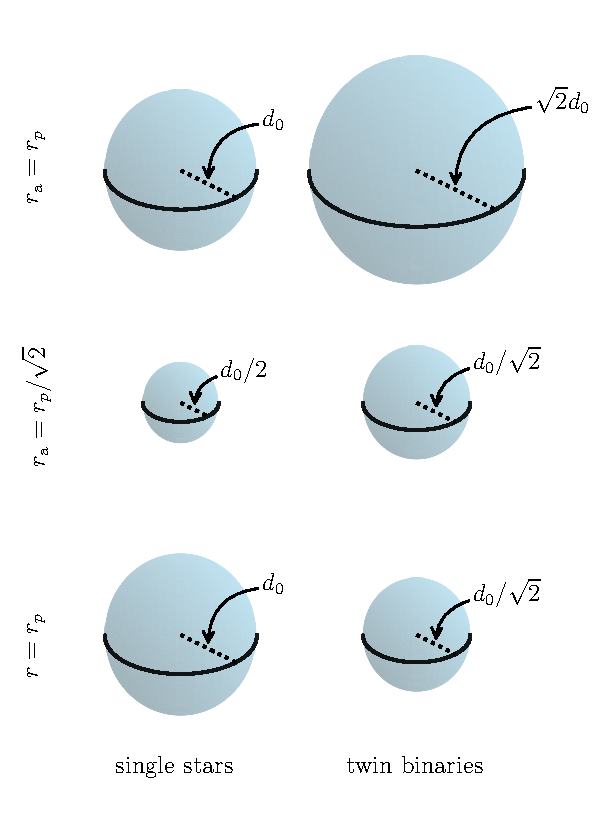
\includegraphics[width=0.6\textwidth]{figures/visualize_volumes.pdf}
    \end{center}
    \caption{
        Cartoon of the searchable volumes for single stars ({\it left}), and 
        twin binaries ({\it right}).
        This model assumes all stars have equal mass and luminosity, and 
        all planets have the same true radius $r=r\p$.
        {\it Top:} At an apparent radius $r\a=r\p$,
        the observer searched twin binaries out to a
        distance $\sqrt{2}\times$ that of single stars.
        Because of dilution, there are no planets in twin binaries with 
        $r\a=r\p$.
        {\it Middle:} At an apparent radius $r\a=r\p/\sqrt{2}$, the 
        maximum searchable distances are half those at $r\a=r\p$. 
        The only detected planets with $r\a=r\p/\sqrt{2}$ orbit twin binaries.
        {\it Bottom:} Planets with a true radius $r=r\p$ are searchable to 
        a maximum distance $d_0$ around singles, and $d_0/\sqrt{2}$ around 
        twin binaries.
    }
    \label{fig:model_1_volumes}
\end{figure}

Since the effects of binarity are most pronounced when the two components are 
similar, we begin by considering a universe in which all planets are 
identical, and all stars are identical except that some fraction of them exist 
in binaries. The goal of this thought experiment is to compare the occurrence 
inferred by observers ignoring binarity with the true occurrence in single 
star systems.

First, what are the possible apparent radii of detected planets?
If the true planet radius is $r=r\p$, then planets in singles will be 
detected with identical apparent radii: $r\a = r\p$.
Conversely, all detections in twin binaries will have apparent radii 
$r\a=r\p/\sqrt{2}$, because they are diluted.
For an unresolved point-source,
\begin{equation}
\delta_{\rm obs}
= \left(\frac{r\a}{R\a}\right)^2
= \left[{r\over R_{\rm host}}\right]^2\times {L_{\rm host} \over L_{\rm 
        sys}(M_1, q)},
\label{eq:delta_obs_general} 
\end{equation}
where $R_{\rm host}$ ($L_{\rm host}$) is the planet-host's stellar radius 
(luminosity), $R\a$ is the apparent stellar radius, $L_{\rm sys}=L_1+L_2 = 
L(M_1) + L(qM_1)$ is the system luminosity, and $q=M_2/M_1$ is the binary mass 
ratio.
We assume that the stellar radius and luminosity are uniquely related to the 
stellar mass.
The observers, with no a priori knowledge of the distance to a system, would 
measure a flux, assume a stellar mass $M\a=M_1$, and estimate a stellar 
radius $R\a = R(M\a)$ and an under-luminous system luminosity of $L_{\rm 
sys,a}(M\a) = L(M\a)$.

The planets will be detected if and only if their host stars are searchable.
For a fixed signal-to-noise floor, there is a maximum searchable 
distance~\citep{pepper_using_2003,pepper_searching_2005}.
From Eq.~\ref{eq:S_N_thresh}, this maximum searchable distance scales as
\begin{equation}
d(\delta_{\rm obs}, L_{\rm sys}) \propto \delta_{\rm obs} \cdot L_{\rm 
    sys}^{1/2}.
\end{equation}
Assuming that stars are uniformly distributed in space, the number 
of searchable stars $N\s$ is then proportional to
\begin{equation}
N\s(\delta_{\rm obs}, L_{\rm sys}) \propto n \delta_{\rm obs}^3 L_{\rm 
    sys}^{3/2},
\label{eq:N_searchable_prop}
\end{equation}
where $n$ is the number per unit volume of {\it e.g.}, single star, or binary 
systems.
We neglect the dependence of $n$ on stellar type.

The searchable volumes for our thought experiment are illustrated 
in Fig.~\ref{fig:model_1_volumes}.
At an apparent radius equal to the true radius ($r\a=r\p$), single stars 
with $d<d_0$ are searchable.
Binaries with $r\a=r\p$ are also searchable, out to $\sqrt{2}d_0$. 
However, in this model no such systems exist; all planets in twin binaries 
have true radii $r=r\p$, and so are observed with apparent radii 
$r\a=r\p/\sqrt{2}$, out to $d_0/\sqrt{2}$.
At an apparent radius of $r\a=r\p/\sqrt{2}$, there could also be planets with 
true radii $r=r\p/\sqrt{2}$ orbiting singles~---~however none of these exist 
in this model.

How many planets are detected?
If we assume that there are $N\s^0(r\a)$ singles that are searchable for 
planets with $r\a$, and that there are $Z_0$ planets per single, then 
single stars contribute
\begin{equation}
n_{\rm det}^0(r\a) = N\s^0(r\a) Z_0 p_{\rm tra} \cdot \delta(r\a - r_p)
\end{equation}
planet detections (per unit $r\a$), where $\delta$ is the Dirac delta function.

We can write similar equations for the binaries.
First though, we define a ratio $\mu \equiv N\s^{\rm b}(r\a) / N\s^0(r\a)$ 
between the number of searchable binary systems and the number of searchable 
singles at any $r\a$.
This quantity is useful because although $N\s^{\rm b}$ and $N\s^0$ vary
as a function of the observed transit depth, $\mu$ remains fixed.
Applying this definition, at $r\a=r\p/\sqrt{2}$, some detections will come 
from primaries,
\begin{equation}
n_{\rm det}^1(r\a) =
\mu N\s^0(r\a) Z_1 p_{\rm tra}
\cdot \delta\left(r\a - \frac{r\p}{\sqrt{2}}\right),
\end{equation}
and some from secondaries,
\begin{equation}
n_{\rm det}^2(r\a) = 
\mu N\s^0(r\a) Z_2 p_{\rm tra}
\cdot \delta\left(r\a - \frac{r\p}{\sqrt{2}}\right),
\end{equation}
where $Z_1$ is the number of planets per primary, $Z_2$ is the number of 
planets per secondary, and $p_{\rm tra}$ is the same for identical stars.
In the case of twin binaries, Eq.~\ref{eq:N_searchable_prop} gives $\mu = 
2^{3/2} n_{\rm b}/n_{\rm s} = 2^{3/2} {\rm BF}/(1-{\rm BF})$, for ${\rm BF}$ 
the binary fraction\footnote{The binary fraction is the fraction of systems in 
a volume-limited sample that are binary. It is equivalent to the multiplicity 
fraction if there are no triple, quadruple, or higher order multiples.
}.

The last item we need to write down the apparent rate density $\Gamma\a(r\a)$ 
is the number of unresolved point-sources on sky, $N_{\rm s,a}$.
Assuming that the apparent stellar radius is fixed, then given the 
apparent planet radius $r\a$,
\begin{equation}
N_{\rm s,a}(r\a) = N\s^0(r\a) \times (1 + \mu)
\label{eq:apparentlysearchable_to_searchable}
\end{equation}
relates the number of apparently searchable point-sources to the number of 
searchable singles.
From the discussion above, it should be clear that there are in fact
$N\s^0(r\a)\times (1 + 2\mu)$ searchable stars at any given $r\a$; the 
observers are under-counting.

Using Eq.~\ref{eq:defn_apparent_rate_density}, the apparent rate density 
computed without considering binarity is
\begin{align}
\Gamma\a(r\a) = 
\frac{1}{1+\mu} Z_0 \cdot
\delta(r\a-r\p)  +
\frac{\mu}{1+\mu} (Z_1 + Z_2) \cdot
\delta\left(r\a-\frac{r\p}{\sqrt{2}} \right).
\label{eq:model_1_apparent_rate_density}
\end{align}
The number of searchable singles at a given apparent radius, 
$N\s^0(r\a)$, makes no appearance.
The observer's errors in Eq.~\ref{eq:model_1_apparent_rate_density} are 
(A) under-counting the number of searchable stars at any apparent radius;
and
(B) inferring radii in binary systems that are all $\sqrt{2}$ too small.

\begin{figure}[!tb]
    \begin{center}
        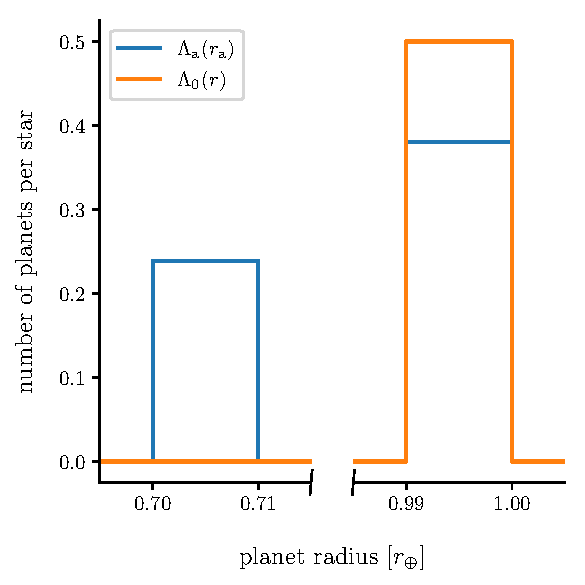
\includegraphics[width=.6\textwidth]{figures/occ_rate_vs_radius_model_1_brokenx.pdf}
    \end{center}
    \vspace{-0.5cm}
    \caption{
        Inferred occurrence rates over $0.01r_\oplus$ bins in planet 
        radius, for a model with identical stars, identical planets, and twin 
        binaries (same as Fig.~\ref{fig:model_1_volumes}).
        We assume a twin binary fraction of ${\rm BF}=0.1$, and that all 
        stars (single, primary, and secondary) host planets at equal 
        rates.
        If the true planet radius is $r\p$, all planets detected in binaries 
        will have apparent radii $r\a = r\p/\sqrt{2}$;
        Eq.~\ref{eq:model_1_apparent_rate_density} gives the normalizations.
        The rate and rate density are related by $\Lambda|_a^b = 
        \int_{a}^{b}\Gamma\,{\rm d}r$.
    }
    \label{fig:occ_rate_model_1}
\end{figure}

To assess the severity of these errors, we need to assume a binary fraction, 
and to know the true number of planets per single, primary, and secondary star 
($Z_0,Z_1,$ and $Z_2$).
For the former,
\citet{raghavan_survey_2010} found a multiplicity 
fraction of 0.44 for primaries with masses from $0.7M_\odot$ to $1.3M_\odot$, 
which we take as a binary fraction. 
``Twin binaries'' are perhaps 10-20\% of the binaries in a volume-limited 
sample, depending on how ``twin'' is defined.
Thus a representative twin binary fraction for this model is ${\rm BF}\approx 
0.05$-$0.1$. 
For the true number of planets per star, we take $Z_0=Z_1=Z_2=0.5$, and plot 
the resulting occurrence rates as a function of planet radius in 
Fig.~\ref{fig:occ_rate_model_1}.

Our point for comparison is the rate density for single stars,
\begin{equation}
\Gamma_0(r) = Z_0 \cdot \delta(r-r\p).
\end{equation}
We define a rate density ``correction factor'', $X_\Gamma$, as the ratio 
of the apparent to single star rate density,
\begin{equation}
X_\Gamma(r) \equiv \left. \frac{\Gamma_a(r\a)}{\Gamma_0(r)} \right|_{r\a 
    \rightarrow r}.
\end{equation}
Continuing in the assumption that the number of planets per single, primary, 
and secondary star are equal, then the rate density 
correction factor at the true planet radius is $1/(1+\mu)$.
This yields a correction of 0.76 if ${\rm BF}=0.1$, and 0.87 if ${\rm 
    BF}=0.05$. Rephrasing the result, if the twin binary fraction were 
$(2^{3/2}+1)^{-1}\approx 0.26$, then the apparent rate at $r\a=r\p$ would be 
half the true rate at $r=r\p$.
For most stellar types, the twin binary fraction is not that high.

An alternative assumption is that secondaries do not host planets. In that 
case, $Z_0=Z_1$, and $Z_2=0$. The correction to the rate density at the true 
planet radius becomes $(1+2\mu)/(1+\mu)^2$.
This evaluates to 0.94 if ${\rm BF}=0.1$, and 0.98 if ${\rm BF}=0.05$.
While it seems unlikely that secondaries are planet-less, 
the fact that $\Gamma\a/\Gamma$ is sensitive to the relative number 
of planets per single, primary, and secondary will become important as we 
proceed.

\subsection{Twin binaries, identical stars, two planet sizes}

A simple extension to the previous example will help us further distinguish 
the detected populations.
Consider now a universe that is the same in every respect to that of 
Sec.~\ref{sec:model_1}, except that half of planets have true radii $r\p$, 
while the other half have true radii $r\p/\sqrt{2}$.
The true rate densities are
\begin{equation}
\Gamma_i(r) = \frac{Z_i}{2} \left[
\delta(r-r\p) + \delta\left(r-\frac{r\p}{\sqrt{2}}\right)
\right], \quad {\rm for}\  i \in \{ 0,1,2 \},
\end{equation}
where as before $i=0$ corresponds to singles, $i=1$ to primaries, and $i=2$ to 
secondaries, and the $Z_i$'s are the number of planets per star of each type.

Following an identical line of reasoning as in Sec.~\ref{sec:model_1}, the 
apparent rate density can be written
\begin{align}
\notag
\Gamma\a(r\a) &=
\frac{1}{2(1+\mu)} \left[
Z_0 \cdot \delta(r\a - r\p)
+
\left[Z_0 + \mu (Z_1 + Z_2)
\right] \cdot \delta\left(r\a - \frac{r\p}{\sqrt{2}}\right) 
\right. \\
&\quad\quad\quad\quad\quad\quad\quad\quad+
\left.
\mu(Z_1 + Z_2) \cdot \delta\left(r\a - \frac{r\p}{2}\right)
\right].
\label{eq:two_radii_twins}
\end{align}
The important qualitative point of this equation is that at $r\a = 
r\p/\sqrt{2}$, two populations contribute.
The first population is singles with $r=r\p/\sqrt{2}$, and the second is twin 
binaries with $r=r\p$.
Both populations are detected out to the same maximum searchable distance.
Just as with Eq.~\ref{eq:apparentlysearchable_to_searchable}, we will have a 
cancellation of $N\s^0(r\a)$ terms, leaving only the $\mu$ weights.




%%%%%%%%%%%%%%%%%%%%%%%%%%%%%%%%%%%%%%%%%%%%%%%%%%%%%%%%%%%%%%%%%%%%%%%%%%%%%%%
%%%%%%%%%%%%%%%%%%%%%%%%%%%%%%%%%%%%%%%%%%%%%%%%%%%%%%%%%%%%%%%%%%%%%%%%%%%%%%%
\section{General formula for apparent occurrence rate}
\label{sec:general_formula}

To generalize the procedure of Sec.~\ref{sec:simplest}, we consider an 
SNR-limited transit survey in which the singles and primaries can have 
arbitrary properties, but their true masses are known by the observer.
We assume that there are some functions $L(M)$ and $R(M)$ that specify a 
star's luminosity and radius in terms of its mass, and that the volume-limited 
binary mass ratio distribution, $f(q)$, is independent of the primary's mass.
We also allow arbitrary true rate densities for singles, primaries, 
and secondaries ($\Gamma_0, \Gamma_1, \Gamma_2$).
We presume that the observers always take the properties of a binary system to 
be those of the primary.

Given this laundry-list of assumptions, a general formula for the apparent 
rate density follows:
\begin{align}
\notag
\Gamma\a(r\a,M\a) &= {1\over 1+\mu(\mathrm{BF}, M\a)}\times
\left\{ \Gamma_0(r\a, M\a)+ 
\frac{{\rm BF}}{1 - {\rm BF}}
\left[ \int \mathrm{d}q \,
       \frac{f(q)}{\mathcal{A}^3}\cdot
       \frac{1}{\mathcal{A}} \Gamma_1\left({r\a\over \mathcal{A}}, 
M\a\right)\,
\right.   
\right. \\
& \quad\quad\quad\quad\quad \left.\left.
+\int {\rm d}q\, \frac{f(q)}{\mathcal{A}^3}\cdot \frac{q}{\mathcal{B}}
    \Gamma_2\left({r\a\over \mathcal{B}}, qM\a\right)\cdot
{R(qM\a) \over R(M\a)}
q^{-1/3} \right]	\right\},
\label{eq:general_Gamma_a}
\end{align}
where ${\rm BF}$ is the volume-limited binary fraction, and $\mathcal{A}$ 
($\mathcal{B}$) is the dilution term for primaries (secondaries).
The dilution terms can be written
\begin{equation}
\mathcal{A}(q, M\a)=\sqrt{L(M\a) \over L_{\rm sys}(M\a, q)}
= (1+q^\alpha)^{-1/2},
\end{equation}
and
\begin{equation}
\mathcal{B}(q, M\a)={R(M\a)\over R(qM\a)}\sqrt{{L(qM\a) \over L_{\rm 
            sys}(M\a, q)} }
= q^{-1} (1+q^{-\alpha})^{-1/2}
\end{equation}
where the latter equalities assume $L\propto M^\alpha \propto R^\alpha$ (the 
former are more general).
The rate densities depend on both apparent radius and mass 
because even if the primaries and singles were to have fixed
mass, the mass of secondaries would vary, and so this dependence cannot be 
immediately omitted.


A derivation of Eq.~\ref{eq:general_Gamma_a} is given in the 
\hyperref[sec:appendix]{Appendix}; here we highlight its qualitative 
features.
The terms inside the curly braces $\{ \ldots \}$ are the sum of 
the apparent rate densities from singles, primaries, and secondaries.
The contribution from singles is not affected by binarity.
In the contributions from primaries and secondaries,
planets with $(r\a, M\a)$ are associated with 
systems of different planetary and stellar properties, as determined
by the mass ratio $q$ of each binary.
This corresponds to true planet radii and stellar masses 
$(r\a/\mathcal{A},M\a)$ for primaries, and $(r\a/\mathcal{B},qM\a)$ for 
secondaries.
These contributions are then integrated over the mass ratio distribution 
including the effect of Malmquist bias, $f(q)/\mathcal{A}^3$, discussed 
further below. Finally, the latter term in the apparent rate density of 
secondaries comes from a correction for the overestimated transit probability.


\paragraph{Ratio of searchable binaries to singles}
We must also specify the exact form of $\mu({\rm BF},M\a)$, the ratio of 
the number of searchable binary systems to singles.
Given the observed signal $\delta_{\rm obs}$ and apparent stellar mass $M\a$, 
recall that the maximum searchable distance for singles and binaries are 
proportional to $\delta_{\rm obs}\cdot L(M\a)^{1/2}$ and $\delta_{\rm 
obs}\cdot [L(M\a)+L(qM\a)]^{1/2}$.
Applying Eq.~\ref{eq:N_searchable_prop},
\begin{equation}
\mu({\rm BF},M\a) = 
\frac{N\s^{\rm b}(r_a)}{N_s^0(r\a)}=
\int_0^1 {n_{\rm b}\over n_{\rm s}}\left[1+{L(qM\a) \over L(M\a)}\right]^{3/2} 
f(q)\,\mathrm{d}q.
\label{eq:mu_general}
\end{equation}
If $\mathrm{BF}$ is independent of $q$, $L \propto M^\alpha$, and $f(q) 
\propto q^\beta$, this simplifies to
\begin{equation}
\mu =\frac{{\rm BF}}{1 - {\rm BF}}\cdot {1\over{1+\beta}}\int_0^1 
\left(1+q^\alpha\right)^{3/2} q^\beta \,\mathrm{d}q,
\label{eq:mu_power_laws}
\end{equation}
which may be written in a closed form using the hypergeometric function.

\begin{figure}[!tb]
    \centering
    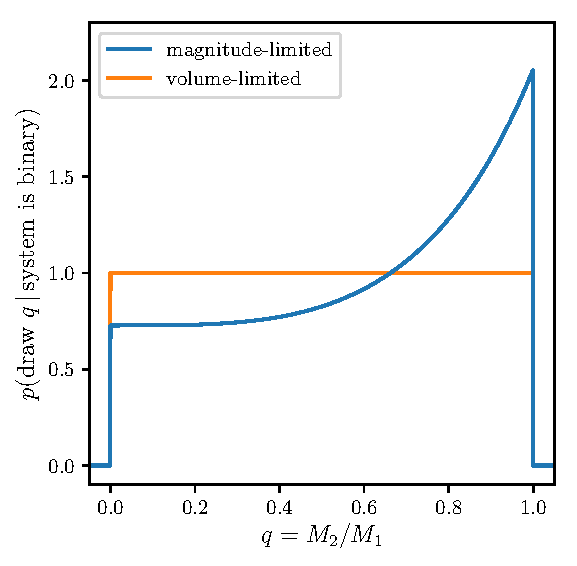
\includegraphics[width=0.6\textwidth]{figures/mass_ratio_distribution.pdf}
    \caption{
        The mass ratio distribution for a magnitude-limited sample of 
        binary stars, in which the underlying volume-limited distribution is 
        uniform, qualitatively similar to {\it e.g.}, 
        \citet{raghavan_survey_2010}'s Fig.~16.
        At a given observed transit depth, the searchable binaries in a 
        transit survey are magnitude-limited.
    }
    \label{fig:q_distribn_mag_limited}
\end{figure}

This can be understood as a Malmquist bias: at fixed observed transit 
depth, for singles and primaries with the same luminosity, binaries are 
searchable to a greater distance.
In particular, the sample of searchable binaries is magnitude-limited.
Given a searchable binary, the probability that it has a mass ratio $q$ 
scales as
\begin{equation}
p({\rm draw\ }q\,|\,{\rm system\ is\ binary}) \propto 
(1+q^\alpha)^{3/2} q^\beta 
\label{eq:Malmquist_bias}
\end{equation}
where $q^\beta$ is the volume-limited probability of drawing a binary of mass 
ratio $q$, and the first term is the Malmquist bias when $L\propto M^\alpha$.
We show this magnitude-limited mass ratio distribution for the $\beta=0$ case 
in Fig.~\ref{fig:q_distribn_mag_limited}.
In Monte Carlo simulations of transit surveys, it is 
important to draw binaries from a correctly biased mass-ratio distribution 
\citep[\textit{e.g.},][]{bakos_hatsouth:_2013,sullivan_transiting_2015,
    gunther_new_2017}.



%%%%%%%%%%%%%%%%%%%%%%%%%%%%%%%%%%%%%%%%%%%%%%%%%%%%%%%%%%%%%%%%%%%%%%%%%%%%%%%
%%%%%%%%%%%%%%%%%%%%%%%%%%%%%%%%%%%%%%%%%%%%%%%%%%%%%%%%%%%%%%%%%%%%%%%%%%%%%%%
%\section{Analytic and Numerical Results}

%\subsection{Model \#1: fixed stars, fixed planets, twin binaries}
\label{sec:model_1}

Since the effects of binarity are most pronounced when the two components are 
similar, we begin by considering a universe in which all planets are 
identical, and all stars are either single or twin stars with otherwise 
identical physical properties.
The occurrence rate density at a planet radius $r$, stellar radius $R$, and 
semimajor axis $a$ for this model is
\begin{equation}
\Gamma(r,R,a) = \sum_i w_i \Lambda_i \delta^3(r_p,R_\star,a_p),
\label{eq:model1_occ_rate_density}
\end{equation}
for $r_p$ and $R_\star$ some fixed planet and stellar radii, $a_p$ a fixed 
semi-major axis, and $\delta$ the Dirac delta function, whose compact
form will be used for brevity.
The occurrence rate over any interval that includes $r_p$, $R_\star$, and 
$a_p$ is
\begin{equation}
\Lambda = \sum_i w_i \Lambda_i = \frac{ \sum_i N_i \Lambda_i }{N_{\rm tot}}.
\end{equation}
The rate is zero over intervals that do not.

To express the rate density of detected planets, $\hat{\Gamma} = \sum 
Q_i\Gamma_i$, we need the detection efficiencies for each system type, which 
are products of the geometric and selection probabilities:
\begin{align}
Q_i(\vec{x}) &= Q_{g,i}(\vec{x}) Q_{c,i}(\vec{x}),\quad {\rm where}\ 
\vec{x}=(r,R,a).
\label{eq:general_detection_efficiency}
\end{align}
Similar to Pepper et al. (2003), but in a new context, we take $Q_c$ as the 
ratio of the number of stars that were searchable to the number of stars that 
were selected.
Assuming a homogeneous distribution of stars, this gives
\begin{equation}
Q_{c,i}(\vec{x}) = \left(
\frac{d_{{\rm det},i}(\vec{x})}{d_{\rm sel}(\vec{x})}
\right)^3,
\end{equation}
for $d_{\rm sel}$ the maximum distance to which surveyed stars are selected, 
and $d_{{\rm det},i}$ the maximum distance to which planets can actually be 
detected about the $i^{\rm th}$ system type.
Note that $d_{\rm sel} \geq d_{{\rm det},i}$.
In a signal-to-noise limited transit survey in which the observer does not 
know which stars are binaries, 
\begin{equation}
d_{\rm sel} \propto (r/R)^2 (L_{\rm sys} T_{\rm dur} A N_{\rm tra})^{1/2},
\end{equation}
for $L_{\rm sys}=L_1(1+\ell)$ the system luminosity, $T_{\rm dur}$ the 
transit duration, $A$ the detector area, and $N_{\rm tra}$ 
the number of observed transits.
However,
\begin{equation}
d_{{\rm det},i} \propto \mathcal{D}_i(r/R)^2 (L_{\rm sys} T_{\rm dur} A N_{\rm 
tra})^{1/2},
\label{eq:d_det_i}
\end{equation}
for the dilution $\mathcal{D}_i$ given by
\begin{align}
\mathcal{D}_i
&=
\left.
\begin{cases}
1 & \text{for } i=0,\ {\rm single} \\
L_1 / L_{\rm sys} = (1+\ell)^{-1}, & \text{for } i=1,\ {\rm primary} \\
\ell L_1 / L_{\rm sys} = (1 + \ell^{-1})^{-1}, & 
    \text{for } i=2,\ {\rm secondary},
\end{cases}
\right.
\label{eq:dilution}
\end{align}
where the light ratio $\ell$ of a given binary is defined as the ratio of 
the luminosity of the secondary to the primary.

The maximum detectable distance to single stars is assumed to be known, and so 
$d_{{\rm sel},0} = d_{{\rm det},0}$.
This means our naive astronomer assumes the fraction of their selected stars 
which are searchable is 1 (this is their ``assumed completeness'').
For binary systems there is a necessary incompleteness, and combining 
Eqs.~\ref{eq:general_detection_efficiency} through~\ref{eq:dilution} yields
\begin{align}
Q_0 &= Q_{g,0}Q_{c,0} = Q_{g,0} \label{eq:detection_efficiency_0}\\
Q_1 &= Q_{g,1}Q_{c,1} = Q_{g,0} (1+q^\alpha)^{-3} \\
Q_2 &= Q_{g,2}Q_{c,2} = Q_{g,0} q^{2/3} (1+q^{-\alpha})^{-3} q^{-5}, 
\label{eq:detection_efficiency_2}
\end{align}
for $Q_{g,0}=R/a$, the transit probability in single star systems.
In Eq.~\ref{eq:detection_efficiency_2}, we have assumed a stellar 
mass-luminosity-radius relation: $R\propto M \propto L^{1/\alpha}$.
The geometric transit probability is $Q_{g,2} = Q_{g,0}q^{2/3}$, and the 
completeness is the latter term of Eq.~\ref{eq:detection_efficiency_2}.
For $q=1$, the $q^{2/3}$ and $q^{-5}$ evaluate to unity, but they will later 
become relevant.

Summarizing, we have written the rate density for each system type
(Eq.~\ref{eq:model1_occ_rate_density}) and the detection efficiency for each 
system type 
(Eq.~\ref{eq:detection_efficiency_0}-\ref{eq:detection_efficiency_2}),
and so have fully specified the rate density of detected planets, 
in addition to the true rate density.


\paragraph{What does an observer ignoring binarity infer?} 
An observer who ignores binarity assumes a detection efficiency 
$\tilde{Q}=Q_0$,
measures a detected planet rate density $\tilde{\Gamma}$, 
and infers an apparent rate density $\Gamma_a$.
Analogous to Eq.~\ref{eq:detected_rate_density},
\begin{equation}
\tilde{\Gamma} = \Gamma_a \tilde{Q}.
\end{equation}
Accounting for dilution, and assuming $q=1$, the apparent rate density is
\begin{equation}
\Gamma_a = 
w_a \Lambda_0 \delta^3(r_p, R_\star, a_p) +
w_b (\Lambda_1 Q_{c,1} + \Lambda_2 Q_{c,2}) 
				\delta^3(r_p/\sqrt{2}, R_\star, a_p),
\end{equation}
for $w_a = N_0/(N_0+N_1)$, and $w_b = N_1/(N_0+N_1)$.
This observer miscounts the number of total searched stars, does not correct 
for incompleteness, and misclassifies the planetary radii because of dilution.

\paragraph{Correction to inferred rate density and inferred rate}

Define a rate density correction factor, $X_\Gamma$, as the ratio of the 
apparent to true rate densities:
\begin{equation}
X_\Gamma \equiv \frac{\Gamma_a}{\Gamma}.
\end{equation}
This factor can be a function of whatever parameters $\Gamma_a$ and $\Gamma$ 
depend on; in this study, the planet radius is most relevant.
For the twin-binaries model,
\begin{equation}
X_\Gamma(r)
=
\frac{w_a \Lambda_0\delta^3(r_p) + 
	w_b(\Lambda_1 Q_{c,1} + \Lambda_2 Q_{c,2}) \delta^3(r_p/\sqrt{2})  }
	{(w_0\Lambda_0 + w_1\Lambda_1 + w_2\Lambda_2)\delta^3(r_p)}
	\label{eq:model1_correction}
	\end{equation}
where $\delta^3(r_p)$ is shorthand for $\delta^3(r-r_p,R-R_\star,a-a_p)$.

If we take the rates $\Lambda_i$ to be equal, applying the definitions of 
the weights gives a rate density correction factor at $r=r_p$ of
$X_\Gamma(r_p) = (1+\mu)^{-1}$, where 
\begin{align}
\mu \equiv \frac{N_1}{N_0} &=
\frac{n_b}{n_s} \left(\frac{d_{\rm sel,b}}{d_{\rm sel,s}}\right)^3 = 
\frac{{\rm BF}}{1-{\rm BF}} (1+\ell)^{3/2},
\label{eq:mu_definition}
\end{align}
for $n_b$ and $n_s$ the number density of binaries and singles in a 
volume limited sample.
Using Raghavan et al. (2010)'s $0.7-1.3M_\odot$ multiplicity fraction as our 
binary fraction\footnote{
The binary fraction is the fraction of systems in a volume-limited sample that 
are binary. It is equivalent to the multiplicity fraction if there are no 
triple, quadruple, or higher order multiples. In that case, ${\rm BF} = n_b / 
(n_s+n_b)$.
}, we set ${\rm BF}=0.44$.
The resulting correction to the rate density is $X_\Gamma(r_p) \approx 0.31$. 
The correction at $r_p/\sqrt{2}$ is infinite.
The numerical realization of this model agrees with these analytic values, and 
its output is shown in Fig~\ref{fig:errcases_model_1}.
%beta = 2.2223355980148636
If instead we assume that $\Lambda_0 = \Lambda_1$, but that $\Lambda_2=0$, we 
find 
$X_\Gamma(r_p) = (1+2\mu)/(1+\mu)^2$.
Taking the same binary fraction, this evaluates to $X_\Gamma(r_p)\approx 0.53$.
Since the correction to the rate is equal to that of rate density, at 
$r=r_p$, the occurrence rate is underestimated by a factor of roughly 2 to 3.

%Note that a correction to the inferred rate, $X_\Lambda$, can be 
%defined analogously:
%\begin{equation}
%X_\Lambda \equiv \frac{\Lambda_a}{\Lambda}.
%\end{equation}
%For this twin binary model, the correction to the rate is the same as that to 
%the rate density.

\subsection{Model \#2: fixed planets and primaries, varying secondaries}
\label{sec:model_2}

The main use of our binary-twin model is to help develop intuition.
We now let the light ratio $\ell = L_2/L_1$ vary across the binary 
population.
It does so because the underlying mass ratio $q=M_2/M_1$ varies.
We keep the primary mass fixed as $M_1$, which is also the mass of all single 
stars.

We parametrize the distribution of binary mass ratios in a volume-limited 
sample as a power law: $p(q)\propto q^\beta$.
For binaries with solar-type primaries\footnote{
Duchene and Kraus (2013), fitting all the multiple systems of Raghavan et al. 
(2010)'s Fig 16, find $\beta = 0.28\pm0.05$ for $0.7<M_\star/M_\odot<1.3$.
Examining only the binary systems of Rhagavan et al 2010, Fig 16, the 
distribution seems roughly uniform, $\beta \approx 0$, except for a claimed 
excess of twin binaries with $q\approx 1$, and an obvious lack of $q<0.1$ 
stellar companions.
}, $\beta$ is probably between 0 and 0.3.
Since we assume stars are a one-parameter family, $R \propto M \propto 
L^{1/\alpha}$, a drawn value of $q$ determines everything about a secondary.

The rate density in this model, $\Gamma(\vec{x})$, is the sum over system 
types of $w_i \Lambda_i p_i(\vec{x})$:
\begin{equation}
\Gamma(\vec{x})
=
\delta^4(r_p,R_\star,a_p,P_p)(w_0 \Lambda_0 + w_1 \Lambda_1)
+ w_2 \Lambda_2 \delta^3(r_p, P_p, a_p) p_2(q),
\label{eq:model2_rate_density}
\end{equation}
where the semimajor axis of the planet must be such that its period is $P_p$, 
and $p_2(q)$ is expressed in terms of the mass ratio instead of the secondary 
star's radius for convenience ($q$ and $R_2$ are interchangeable).
The probability that a secondary hosts a planet, as a function of the mass 
ratio, is
\begin{align}
p_2(q) &= p({\rm has\ planet}\,|\,{\rm secondary\ with\ }q) \times
          p({\rm secondary\ with\ }q)
          \\
p_2(q) &\propto q^{\gamma + \beta} (1+q^\alpha)^{3/2}.
\label{eq:model_2_p_2}
\end{align}
We take first term, $p({\rm has\ planet}\,|\,{\rm secondary\ with\ }q)$, as a 
power law of $q$ with exponent $\gamma$.
For the second term, since the selected sample at a given $(r,P,a)$ is
magnitude-limited, $p({\rm secondary\ with\ }q)$ 
is the product of the volume limited probability, $q^\beta$, and a 
Malmquist-like bias, $(1+q^\alpha)^{3/2}$.
We note that various authors (probably ourselves included) have incorrectly 
drawn from volume-limited binary distributions in Monte Carlo simulations of 
transit surveys (Sullivan et al 2015, Bakos et al 2012, Guenther et al 
2017, Bouma et al 2017).
The correct distribution for a magnitude-limited selection is shown in 
Fig.~\ref{fig:q_distribn_mag_limited}.

The occurrence rate corresponding to Eq.~\ref{eq:model2_rate_density}'s rate 
density for a desired volume of phase space $\Omega_{\rm desired}$ is given by 
Eq.~\ref{eq:occ_rate}.
Specifying the desired mass ratios of interest as $q_{\rm min} < q < q_{\rm 
max}$, this simplifies to
\begin{equation}
\Lambda = 
\frac{N_0 \Lambda_0 + N_1 \Lambda_1 + N_2 \Lambda_2 f_2}
{N_{\rm tot}},
\end{equation}
for
\begin{equation}
f_2 \equiv
\left(
\int_{q_{\rm min}}^{q_{\rm max}} p_2(q) \,{\rm d}q
\right)
\cdot
\left(
\int_{0}^{1} p_2(q) \,{\rm d}q
\right)^{-1}.
\end{equation}

The detected rate density, $\hat{\Gamma} = \sum_i Q_i \Gamma_i$, will be 
specified by the detection efficiencies for each type of system.
These are identical to 
Eqs.~\ref{eq:detection_efficiency_0}-\ref{eq:detection_efficiency_2}.
The detection efficiency for secondaries (Eq.~\ref{eq:detection_efficiency_2}) 
includes the transit probability from the smaller stellar radius, and combines 
dilution, the transit duration, and stellar radius for the completeness
probability.

\paragraph{What does an observer ignoring binarity infer?}
As a reminder, the apparent rate density is found by correcting the detected 
apparent rate density for the transit probability:
$\Gamma_a = \tilde{\Gamma} Q_{g,0}^{-1}$.
The observer's errors are as follows:
\begin{enumerate}
    \item The true planetary radii $r$ are interpreted as apparent radii $r_a$.
    The apparent radii depend on the system type:
    \begin{align}
    r_a
    &=
    \left.
    \begin{cases}
    r_p (1+q^\alpha)^{-1/2} & \text{for } i=1,\ {\rm primary} \\
    r_p (1+q^{-\alpha})^{-1/2} q^{-1}, & \text{for } i=2,\ {\rm secondary}.
    \end{cases}
    \right.
    \label{eq:model2_ra}
    \end{align}
    The factor of $q^{-1}$ for the secondary case accounts for the observer 
    assuming that the host star is the primary.
    \item The completeness fraction is miscalculated for any stars in binary 
    systems.
    \item The selected and searchable stars are miscounted.
\end{enumerate}

To write the apparent rate density as a function of the apparent 
radius $r_a$, we marginalize out the planet period, semimajor axis, and 
stellar radius (or equivalently the mass ratio, for binaries):
\begin{equation}
\Gamma_a(r_a) =
w_a \Lambda_0 \delta(r_p)
+
w_b \Lambda_1 I_1(r_a)
+
w_b \Lambda_2 I_2(r_a),
\label{eq:model2_Gamma_a}
\end{equation}
where the detection efficiencies are given in 
Eqs.~\ref{eq:detection_efficiency_0}-\ref{eq:detection_efficiency_2}, and as 
in the first model, $w_a=N_0/(N_0+N_1)$, $w_b=N_1/(N_0+N_1)$. The ratio of 
primaries to singles, $\mu$, is now given by a variant of 
Eq.~\ref{eq:mu_definition}:
\begin{equation}
\mu \equiv \frac{N_1}{N_0} = \frac{\rm BF}{1 - {\rm BF}} \left(2^{3/2} - 
\int_{1}^{\sqrt{2}} u^2 (u^2 -1)^{1/\alpha} \,{\rm d}u\right),
\label{eq:mu_model_2}
\end{equation}
where the latter dimensionless integral is easily found numerically.
The $I_1(r_a)$ and $I_2(r_a)$ terms marginalize over the joint distribution of 
apparent radius and mass ratio:
\begin{align}
I_i(r_a) &= 
\int_0^1 p({\rm has\ detected\ planet}, r_a, q | {\rm star\ is\ type\ }i)
    \,{\rm d}q,
\quad
{\rm for}\ i\in\{1, 2\}, \\
&=
\int_0^1 
    p({\rm has\ detected\ planet} | r_a, q, {\rm star\ is\ type\ }i) 
    \nonumber\\
    &\quad\quad\quad\quad\times p(r_a | q, {\rm star\ is\ type\ }i)
    \,p(q | {\rm star\ is\ type\ }i)
\,{\rm d}q.
\end{align}
The first term is the detection efficiency; the second is a $\delta$-function 
of the apparent radius; the last is the mass ratio distribution given by 
Eq.~\ref{eq:model_2_p_2}.
The analytic solution for $i=1$ is
\begin{equation}
I_1(r_a) = \frac{1}{\mathcal{N}_1} \left(\frac{r_p}{r_a}\right)^{-3}
\left( \left(\frac{r_p}{r_a}\right)^2 -1  
    \right)^{\frac{\gamma+\beta}{\alpha}},
\quad {\rm for}\ r_p/\sqrt{2} < r_a < r_p,
\end{equation}
where $\mathcal{N}_1$ is the normalization term of the binary mass ratio 
distribution (Eq.~\ref{eq:model_2_p_2}): $\mathcal{N}_1 = \int_0^1 
q^{\gamma+\beta} (1+q^\alpha)^{3/2} {\rm d}q$.

For $i=2$, there is no analytic solution, because evaluating the integral 
requires imposing the constraint that $r_a  = r_p 
(1+q^{-\alpha})^{-1/2}q^{-1}$. This equation can be re-written
\begin{equation}
\left(\frac{r_p}{r_a}\right)^2 = q^2 + q^{-\alpha + 2},
\end{equation}
which has no analytic solution except for special values of $\alpha$, the 
mass-luminosity exponent.
For $\alpha=3.5$, our nominal case, semianalytic solutions can be found.

Since our main interest is in understanding the qualitative behavior 
of the solutions, we focus on a few analytic limiting cases, and then 
proceed numerically.


\paragraph{Correction to inferred rate density}
Recall that the rate density correction factor, $X_\Gamma$, is the ratio of 
the apparent to true rate densities.
We consider a ``nominal model'' in which the stellar population is similar to 
Sun-like stars in the local neighborhood:
${\rm BF}=0.44$, $\alpha=3.5$, $\beta=0$.
Our default assumption is also that the occurrence of planets is independent 
of stellar mass ($\gamma=0$), so secondaries have the same occurrence rate as 
primaries and single stars.
Under these assumptions, the planetary rate density is
\begin{equation}
\Gamma(r) \approx \delta(r_p) \left( \Lambda_0 + \Lambda_1 + 
\Lambda_2 \right) / 3,
\label{eq:model2_Gamma_r}
\end{equation}
where the coefficients of $1/3$ are accurate to within one percent of the true 
coefficients.
Ignoring binarity, the observer finds an apparent rate density
\begin{equation}
\Gamma_a(r) = c_0 \Lambda_0 \delta(r_p)
             +c_1 \Lambda_1 I_1(r_a)
             +c_2 \Lambda_2 I_2(r_a),
\label{eq:model2_Gamma_a_r}
\end{equation}
for $c_0\approx 0.49$, $c_1\approx 0.32$, $c_2\approx 0.03$.
%171011_integrals.nb
Evaluating the correction term at $r=r_p$, since $\lim_{q\rightarrow0} 
p_i(r_a)=0$ for $i\in\{1,2\}$,
\begin{equation}
X_\Gamma(r=r_p) \approx \frac{3c_0 \Lambda_0}{\Lambda_0+\Lambda_1+\Lambda_2}.
\end{equation}
If all the rates are equal, $X_\Gamma(r=r_p)\approx0.49$.
If there are no planets around the secondaries, $X_\Gamma(r=r_p)\approx0.74$.

We also run this model in our numerical simulation.
The results are shown in Figs.~\ref{fig:errcases_model_2_linear} 
and~\ref{fig:errcases_model_2_log}.
They produce the same correction factors as predicted analytically.
They also show a peak in the inferred rate at $r_p/\sqrt{2}$ from 
secondaries.
This effect requires the observer to incorrectly estimate the host star's 
radius; if they somehow knew the host star's radius, but did not correct for 
binary dilution, the peak would instead be at an apparent radius of 0.

To summarize, dilution produces a spectrum of apparent planetary radii. In 
this model, this produces overestimated rates everywhere except where there 
are actually planets, where the rate is underestimated by a factor of 2.

\subsection{Model \#3: Fixed primaries, varying planets and secondaries}
\label{sec:model_3}

In this model, as in the previous one, all single and primary stars have 
identical properties.
Only the secondaries have masses, radii, and luminosities that vary between 
systems: $M\propto R \propto L^{1/\alpha}$.
The radii of planets are assigned independently of any host system
property, and are sampled from an intrinsic radius distribution, which we take 
as
\begin{align}
p_r(r)
&\propto
\left.
\begin{cases}
r^\delta & \text{for } r\geq 2r_\oplus \\
{\rm constant} & \text{for } r\leq2r_\oplus.
\end{cases}
\right.
\label{eq:model3_radius_distribution}
\end{align}
Following Howard et al. (2012)'s measurement, we take $\delta = -2.92$.
Our ``nominal model'' remains the same: the binary fraction is 0.44, 
$\alpha=3.5$, $\beta=\gamma=0$.
We take $Z_i$, the occurrence rate integrated over all planet radii for the 
$i^{\rm th}$ system type, to be equal for singles, primaries, 
and secondaries. 

For this model, we forgo analytic development and focus only on numerics.
The occurrence rates are shown as a function of planet radius in 
Fig.~\ref{fig:errcases_model_3_log}.
For the assumed planetary and stellar distributions, the inferred rate is 
underestimated over all radii.

\begin{figure}[!tb]
    \centering
    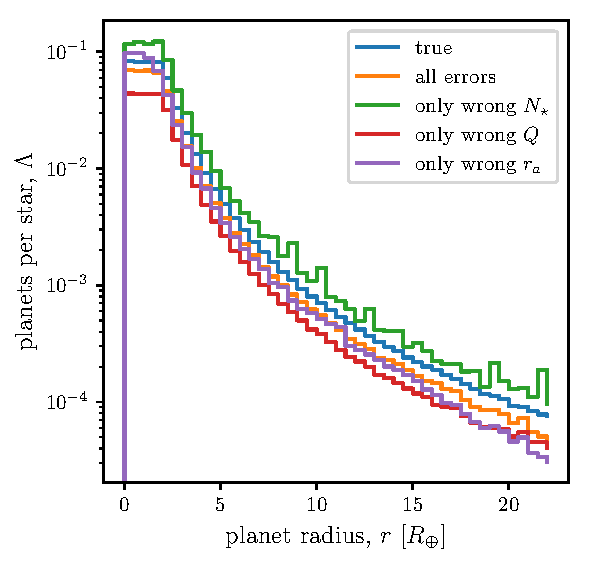
\includegraphics[width=.6\textwidth]{figures/errcases_rate_density_vs_radius_logs_model_3.pdf}
    \caption{
        Inferred planet occurrence rates as a function of planet radius in 
        Model 
        \#3.
        This model has fixed primaries and single stars, but varying 
        secondaries.
        The true planet radius distribution is a power law with exponent 
        $-2.92$ 
        above $2R_\oplus$, below which it is uniform (e.g., Howard et al., 
        2012).
    }
    \label{fig:errcases_model_3_log}
\end{figure}

\paragraph{Hot Jupiter Occurrence Rates}
Taking Fig.~\ref{fig:errcases_model_3_log} and counting the number of planets 
per star with $r>8r_\oplus$, we can compare the true and inferred hot Jupiter 
occurrence rates.
Under the above assumptions, the true rate is 9.1 hot Jupiters 
per thousand stars.
The inferred rate is 6.9 per thousand stars.
This means that the inferred rate underestimates the true rate by a 
multiplicative factor of $\sim\!1.3$.

However, this result only applies under the assumption that $Z_0 = 
Z_1 = Z_2$.
If hot Jupiters are less common around lower mass stars, it would be more 
sensible to consider $Z_2<Z_0$, while letting single stars and 
primaries host planets at the same rate.
Therefore in Fig.~\ref{fig:HJ_correction_inputrate_vs_HJratevalues} we let 
$Z_2$ vary, and show the resulting inferred and true hot Jupiter 
($r>8r_\oplus$) rates.
The result is that the inferred rate is nearly independent of 
$Z_2$~--~this is because most ($<1/10$) secondaries are not searchable, 
and so their completeness fraction is much smaller than that of primaries or 
single stars.
This means far fewer detected hot Jupiters orbit secondaries, and so they 
hardly affect the inferred rate.
While the ``true rate'' across the entire population is linearly dependent on 
$Z_2$, the rate around 
singles and primaries (green line) is independent of that around secondaries.
Assuming that RV surveys are measuring the true rate around single stars (or 
primaries), this suggests that binarity might contributes to the 
HJ rate discrepancy at the $\sim 0.2\%$ level, independent of the HJ rate 
around secondaries.


\begin{figure}[!tb]
    \centering
    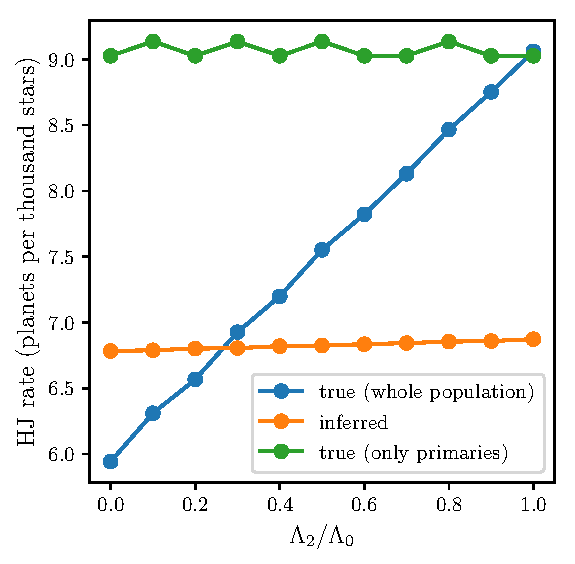
\includegraphics[width=.6\textwidth]{figures/HJ_correction_inputrate_vs_HJratevalues.pdf}
    \caption{
        $X_i$ is the occurrence rate integrated over all possible phase 
        space for the $i^{\rm th}$ system type. $Z_2/Z_0=1$ 
        corresponds to an equal number of planets per secondary as per single 
        star;
        $Z_2/Z_0=0$ corresponds to secondaries not having any 
        planets.
        In our Model \#3, though the true HJ occurrence rate 
        is highly dependent on $Z_2$, 
        the inferred rate hardly depends on whether secondaries have HJs.
        This means that the ``correction factor'' between the inferred rate 
        and the true rate around single stars is underestimated by a 
        multiplicative 
        factor of $\approx1.3$, independent of the HJ rate around secondaries.
        The ``HJ rate'' is the summed rate from     
        Fig.~\ref{fig:errcases_model_3_log} above $8r_\oplus$.
    }
    \label{fig:HJ_correction_inputrate_vs_HJratevalues}
\end{figure}


\paragraph{The Rate of Earth Analogs}
The rate (density) of Earth-like planets orbiting Sun-like stars has 
been independently measured by Youdin, Petigura, Dong \& Zhu, 
Foreman-Mackey et al., and Burke et al., (2011, 2013, 2013, 2014, and 2015 
respectively).
These efforts have found that the one-year terrestrial planet occurrence rate 
varies between $\approx 0.03$ and $\approx 1$ per Sun-like star, depending on 
assumptions that are made when retrieving the rate (Burke et al. 2015's 
Fig.~17).

Our model does not explicitly include the rate density's period-dependence, 
because stellar binarity does not appreciably bias the period-dependence of 
occurrence rates measured by transit surveys\footnote{
    Note that stellar binarity does bias the {\it intrinsic} planet 
    occurrence as a function of planetary and binary periods. This is expected 
    from dynamical stability limits in $\geq$3 body systems, and has been 
    observationally confirmed (theory by Holman \& Wiegert 1999, and others 
    including Gongjie; confirmation from Wang et al 2014a, 2014b, Kraus et al 
    2014). 
    However our statement is that inferred rates as a function of planet     
    period should be negligibly affected by this, given the geometric bias 
    against long-period transit detections, and the fact that the period 
    distribution of solar-type binaries peaks at $\approx 100\,{\rm years}$ 
    (Raghavan et al 2010, Fig.~13).
}.
Instead, it allows us to evaluate the difference in the apparent and true rate 
as a function of radius 
(Fig.~\ref{fig:errcases_model_3_log}).
At Earth's radius, the result is that the inferred rate is $0.84\times$ the 
true rate around single stars, assuming that the $Z_i$'s are equal.
Similar to the above case of the hot Jupiters, if we vary the true $Z_2$ 
while keeping $Z_0 = Z_1$, the ratio of the inferred to true rate 
around single stars hardly 
changes by only a few percent (shown in 
Fig.~\ref{fig:earth_inputrate_vs_etaearthratevalues}).
The ratio of the inferred to the true rate, $(\Lambda_{\rm 
inferred}/\Lambda)_{r=r_\oplus}$ varies substantially, but by at most $50\%$ 
in the (unrealistic) limiting case that secondaries do not host planets.


\begin{figure}[!tb]
    \centering
    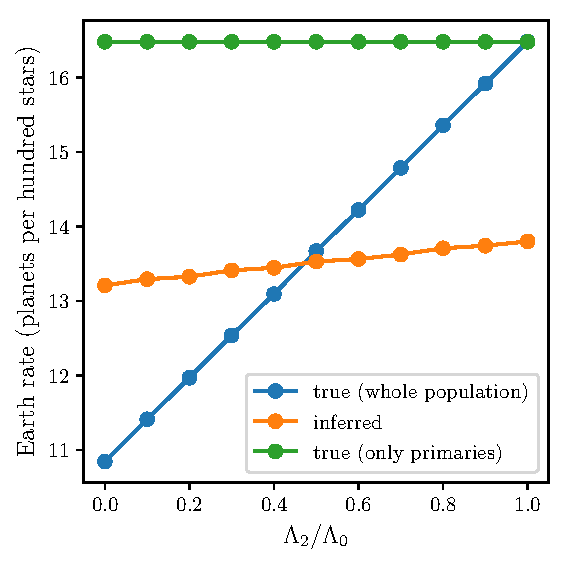
\includegraphics[width=.6\textwidth]{figures/earth_inputrate_vs_etaearthratevalues.pdf}
    \caption{
        Same as Fig.~\ref{fig:HJ_correction_inputrate_vs_HJratevalues}, but 
        for Earth-sized planets.
        The absolute values given on the $y$-axis found by summing the rate 
        from Fig.~\ref{fig:errcases_model_3_log} for planetary radii from 
        $0.5$ to $1.5r_\oplus$ (this is a toy model, and they do not reflect 
        an actual determination of $\eta_\oplus$).
        The relative values show that the inferred rate for Earths is roughly 
        independent of the occurrence rate (integrated over all radii) around 
        secondaries.
        However, it is systematically lower than the true rate around single 
        and primary stars, by $\approx 20\%$.
    }
    \label{fig:earth_inputrate_vs_etaearthratevalues}
\end{figure}

\section{More complicated transit survey models}
\label{sec:more_complicated}
The following section applies our general equation for the apparent rate 
density (Eq.~\ref{eq:general_Gamma_a}) to study binarity's effects in regimes 
of observational interest.
In general, we will write the rate density for each type of star, 
$\Gamma_i(r)$, as the product of a shape function and a constant:
\begin{equation}
\Gamma_i(r) = Z_i f_i(r), \quad {\rm for\ }i\in\{0,1,2\},
\end{equation}
where as always, $i=0$ corresponds to single stars, $i=1$ to primaries of 
binaries, and $i=2$ to secondaries of binaries.
The shape function is normalized to unity.
The $Z_i$'s are each system type's occurrence rate $\Lambda_i$, integrated 
over all planetary radii. In other words, they are number of planets per 
single, primary, or secondary star.
This section will consider the effects of varying both $f_i(r)$ and also the
relative values of the $Z_i$'s.

%%%%%%%%%%%%%%%%%%%%%%%%%%%%%%%%%%%%%%%%%%%%%%%%%%%%%%%%%%%%%%%%%%%%%%%%%%%%%%%
\subsection{Power law planet radius distributions}
\label{sec:model_2}

\subsubsection{Twin binaries}
We begin introducing realism by keeping all binaries as twins, but letting the 
radius distribution of planets vary.
Specifically, we take
\begin{equation}
\Gamma_i(r) = Z_i f(r) = Z_i r^\delta/\mathcal{N}_r,
\end{equation}
for $f(r)$ the radius shape function, and $\mathcal{N}_r$ the shape function's 
normalization.
The resulting apparent rate density is quite similar to that of the twin 
binary, fixed-planet case (Eq.~\ref{eq:model_1_apparent_rate_density}), except 
for a slightly different radius dependence and normalization:
\begin{equation}
\Gamma\a(r\a) = \frac{r\a^\delta}{\mathcal{N}_r} \left[
\frac{Z_0}{1+\mu}
+
2^{\frac{\delta+1}{2} } \frac{\mu}{1+\mu} \left(Z_1 + Z_2
\right)
\right].
\label{eq:model5_apparent_rate_density}
\end{equation}
As in Sec.~\ref{sec:model_1}, $\mu = 2^{3/2} {\rm BF}/(1-{\rm BF})$.
If the $Z_i$'s are equal, the ``correction factor'' relative to the rate 
density for singles becomes quite simple:
\begin{align}
\left. \frac{\Gamma\a(r\a)}{\Gamma_0(r)} 
\right|_{r\a\rightarrow r}
&=
\frac{1 + 2^{\frac{\delta+3}{2}}\mu}{1 + \mu}.
\label{eq:power_law_correction}
\end{align}
For the case of ${\rm BF}=0.1$, $\mu\approx 0.153$. Taking $\delta=-2.92$ from 
\citet{howard_planet_2012},  we get a correction factor $\Gamma\a/\Gamma_0 = 
1.004$.
In other words, the apparent rate density is an {\it over}estimate compared to 
the rate density of single stars, with a relative difference $\delta \Gamma_0 
= |\Gamma_0 - \Gamma\a | / \Gamma_0$ of 0.4\%.
This is quite a small effect!
Note though that it could change if the $Z_i$'s are not equal.
Also, the power law radius distribution $f(r) \propto r^\delta$ diverges for 
$\delta < 0$; \citet{howard_planet_2012}'s results indicate that this
approximation is good for $r\a\gtrsim 2r_\oplus$.
Similarly, it is nonsensical for $f(r)$ to be finite above some upper radius 
limit $r_u$, perhaps around $\approx 24r_\oplus$, based on the most inflated 
hot Jupiters.
An upper cut-off of $r_u$ would lead to smaller values of $\Gamma(r\a)$ 
down to $r_u/\sqrt{2}$, compared to an intrinsic power law without the cut-off.
We are not particularly interested in this effect; there are better 
models for hot Jupiter occurrence rates that we will discuss in 
Sec.~\ref{sec:further_models}.
If the assumptions behind this model (listed in 
Sec.~\ref{sec:general_formula}) are at all applicable in real transit surveys, 
this suggests that for $2r_\oplus \lesssim r\a \lesssim 17r_\oplus$, 
binarity's impact on derived occurrence rates is quite small.



%%%%%%%%%%%%%%%%%%%%%%%%%%%%%%%%%%%%%%%%%%%%%%%%%%%%%%%%%%%%%%%%%%%%%%%%%%%%%%%
\subsubsection{Varying binaries}
\label{sub:powerlaw_varying_binaries}

To check whether non-twin binaries change the above result, we now assume 
$f(q) = q^\beta/\mathcal{N}_q$, for $\mathcal{N}_q$ the normalization.
This changes $\mu$ (Eq.~\ref{eq:mu_general} simplifies to 
Eq.~\ref{eq:mu_power_laws}).
It may also affect the rate density, which could be a function of the 
(varying) stellar mass.
Absorbing this dependence into a power law as well,
\begin{equation}
\Gamma_i(r,M) = Z_i \times \frac{r^\delta}{\mathcal{N}_r} \times
\frac{M^\gamma}{\mathcal{N}_M},
\end{equation}
where $Z_i$ is dimensionless, and the normalization constants carry 
the units (each side has units $[r^{-1} M^{-1}]$).
We assume that stars are a one-parameter family, given by $R \propto M \propto 
L^{\frac{1}{\alpha}}$, so that a given value of $q$ determines everything 
about a secondary.

We are mostly interested in the apparent rate density's radius dependence.
Marginalizing Eq.~\ref{eq:general_Gamma_a} over apparent stellar mass, we find
that when $Z_0=Z_1=Z_2$,
\begin{align}
X_\Gamma &\equiv \left. \frac{\Gamma\a(r\a)}{\Gamma_0(r)} 
\right|_{r\a\rightarrow r} \\
&=
\notag
\frac{1}{1+\mu}
\left[1 + \frac{1}{\mathcal{N}_q} \frac{{\rm BF}}{1-{\rm BF}}\times 
\left(
\int {\rm d}q\,q^\beta (1+q^\alpha)^{\frac{\delta+4}{2}} +
\right.
\right. \\
&\quad\quad\quad\quad\quad\quad\quad\quad\quad\quad
\left.\left.
\int {\rm d}q\,q^{\beta+\gamma+\delta+\frac{5}{3}} 
(1+q^\alpha)^{\frac{3}{2}}
(1+q^{-\alpha})^{\frac{\delta+1}{2}}
\right)\right].
\label{eq:powerlaw_vary_binary}
\end{align}

For $\alpha = 3.5$, $\beta=0$, $\gamma=0$, $\delta=-2.92$, the 
summed integrals in Eq.~\ref{eq:powerlaw_vary_binary} give $(\ldots)\approx 
1.50249$. %171211_model_integrals.nb
For ${\rm BF}=0.44$, this yields $\Gamma\a/\Gamma_0 = 1.048$; the
relative difference between the apparent rate density and the rate density 
around singles is 4.8\%.
This indicates that considering only twin binaries gave us correct 
intuition: for a power-law radius distribution 
($2r_\oplus \lesssim r\a \lesssim 17r_\oplus$) in which there are the same 
number of planets orbiting singles, primaries, and secondaries, binarity 
influences apparent planet occurrence rates around Sun-like stars at the 
$\sim$few percent level.




%%%%%%%%%%%%%%%%%%%%%%%%%%%%%%%%%%%%%%%%%%%%%%%%%%%%%%%%%%%%%%%%%%%%%%%%%%%%%%%
\subsection{Fixed primaries, varying secondaries, broken power-law planets}
\label{sec:model_3}

\begin{figure}[!t]
    \centering
    \epsscale{1.15}
    \plottwo{figures/int_rate_density_vs_radius_model_3_rpu_22.5_manyZs.pdf}{figures/int_occ_rate_vs_radius_model_3_rpu_22.5_manyZs.pdf}
    \caption{
        {\it Left:} rate density and {\it right:} rate (over $0.5r_\oplus$ 
        bins) as a function of planet radius for the distribution specified by 
        Eq.~\ref{eq:model3_radius_distribution}. 
        This model assumes that the true properties of all the singles and 
        primaries are known to the observer, and that the volume-limited mass 
        ratios of secondaries are drawn from a uniform distribution. We use an 
        arbitrary normalization of $Z_0=Z_1=0.5$ throughout.
        The rate and rate density are related by $\Lambda|_a^b 
        = \int_{a}^{b}\Gamma\,{\rm d}r$.
    }
    \label{fig:occ_rate_model_3_log}
\end{figure}

Though the details of the true radius distribution $\Gamma_i(r)$ at 
$r<2r_\oplus$ are currently an active topic of research, we can consider how 
binarity affects this regime under various reasonable assumptions.
For instance, assume that the true radius shape function is
\begin{align}
f(r)
&\propto
\left.
\begin{cases}
r^\delta & \text{for } r\geq 2r_\oplus \\
{\rm constant} & \text{for } r\leq2r_\oplus.
\end{cases}
\right.
\label{eq:model3_radius_distribution}
\end{align}
As in the previous model, we assume that the observers know the true 
properties of all singles and primaries. The masses, radii, 
and luminosities of stars vary as $R \propto M \propto L^{\frac{1}{\alpha}}$.
Our ``nominal model'' remains the same: 
$\alpha=3.5$, $\beta=\gamma=0$, $\delta=-2.92$.

At apparent radii $r\a > 2r_\oplus$, the results of this model are the same as 
those from Sec.~\ref{sub:powerlaw_varying_binaries}.
For $r\a < 2r_\oplus$, the equations are tedious, but still tractable.
For simplicity, we insert Eq.~\ref{eq:model3_radius_distribution} into 
Eq.~\ref{eq:general_Gamma_a}, and integrate using a computer 
program. We refer the interested reader to our online 
implementation\footnote{\url{https://github.com/lgbouma/binary_biases}}.
The output is validated against analytic predictions in the $r\a > 
2r_\oplus$ and the $r\a < 2r_\oplus/\sqrt{2}$ regimes, and is plotted in
Fig.~\ref{fig:occ_rate_model_3_log}.


\paragraph{The rate of Earth analogs}
The immediately arresting result there is a ``bump'' in the apparent rate 
density at $r\a < 2r_\oplus$: the true rate for singles is less than the 
inferred rate.
For the case in which secondaries host as many (half as many) planets as 
single stars, this means an overestimate of the absolute occurrence rate by 
$\approx 50\%$ ($\approx 25\%$).
The ``bump'' exists even for the $Z_2/Z_0=0$ case as a $\approx 10\%$ effect.
Evidently, the magnitude of this error depends strongly on the prevalence of 
planets around secondaries.

\paragraph{Hot Jupiter occurrence rates}
Taking Fig.~\ref{fig:occ_rate_model_3_log} and integrating the rate density, 
we can compare the apparent hot Jupiter 
occurrence rate with the true rate for singles.
In the most extreme case of $Z_2/Z_0=0$, we find that $\Lambda_{{\rm 
HJ},0}/\Lambda_{\rm HJ,a} = 1.13$, where
\begin{equation}
\Lambda_{\rm HJ,a} = \int_{8r_\oplus}^{\infty} \Gamma\a(r)\,{\rm d}r,
\end{equation}
and similarly for $\Lambda_{\rm HJ,0}$.
%occ_rate_vs_radius_model_3_withtext_Zsub2_0.00_rpu_22.5.pdf
If $Z_2/Z_0>0$, binarity affects the apparent hot Jupiter rate less: when 
$Z_2/Z_0=0.5$, we find $\Lambda_{{\rm HJ},0}/\Lambda_{\rm HJ,a} = 1.06$

\paragraph{Fraction of detected planets from a given source}

\begin{figure}[!t]
    \centering
    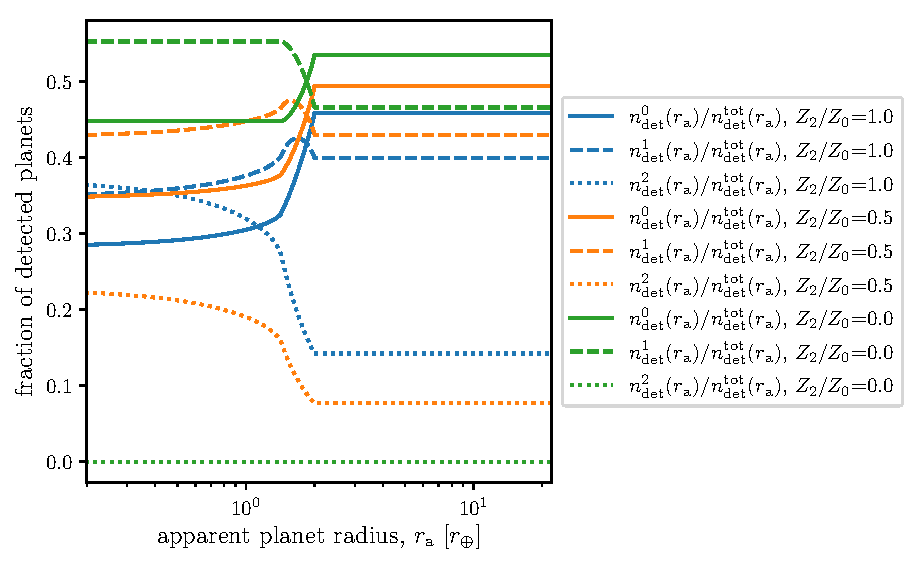
\includegraphics[width=\textwidth]{figures/ndet_vs_radius_logx_model_3_fraclines_rpu_22.5_manyZs.pdf}
    \caption{
        Fraction of detected planet at a given apparent planet radius coming 
        from singles (solid lines), primaries (dashed lines), and secondaries 
        (dotted lines).
        Three different values for $Z_2/Z_0$ are selected: $1$ (blue), $0.5$ 
        (orange), $0$ (green).
        The assumed true planet radius distribution is a broken power-law
        (Eq.~\ref{eq:model3_radius_distribution}; same as 
        Fig.~\ref{fig:occ_rate_model_3_log}).
    }
    \label{fig:frac_model_3}
\end{figure}

It would be nice to improve our intuition for how much the secondaries matter.
We have the understanding that for a given true planet radius, secondaries 
have a much smaller searchable volume than primaries or singles.
Does this necessarily imply that if we are given a detected planet with some 
apparent radius $r\a$, which is then observed by high-resolution imaging to 
exist in a binary, that the planet probably orbits the primary?

We explore this quantitatively in Fig.~\ref{fig:frac_model_3}.
The lines in this figure are computed using the expressions given in the 
appendix for the number of detections coming from singles, primaries, and 
secondaries (Eqs.~\ref{eq:n_det_0},~\ref{eq:n_det_1}, and~\ref{eq:n_det_2}).

In short, the answer to our question is ``it depends on the number of planets 
orbiting secondaries, and also on the apparent radius of the detected planet''.
In the scenario that high-resolution imaging finds a system with $r\a > 
2r_\oplus$ in a binary, roughly $\sim 2.5\times$ more detected planets orbit 
primaries than secondaries, for the $Z_2/Z_0=1$ case.
For the $Z_2/Z_0=0.5$ case, $\sim 5\times$ more detected 
planets orbit primaries than secondaries.
So, relative to the cutoff in the intrinsic rate density, detected planets in 
binaries with large apparent radii are more likely to orbit the primary.

The situation for $r\a < 2r_\oplus$ is more nuanced.
For the $Z_2=0$ and $Z_2/Z_0=0.5$ cases, detected planets in binaries are 
still always more likely to orbit the primary.
However, if there are as many planets orbiting the secondaries as the 
primaries, then there is a turn-over radius, $\approx 0.4r_\oplus$, 
beyond which more of the detected planets in binaries come from secondaries: 
they have all been ``diluted down'' from larger true planetary radii!
Although this (apparent) radius is at the limit of current detection 
sensitivities, this effect will be interesting for future instruments to 
investigate.

Further, Fig.~\ref{fig:frac_model_3} shows that going from apparent 
radii of $2r_\oplus$ to $\approx 1.4r_\oplus$, the fraction of detected 
planets with binary companions increases by $\approx 6-12\%$, depending on the 
assumed value of $Z_2/Z_0$.
Let the fraction of total detected planets from primaries at a given 
apparent radius be $F_1(r\a)$, and from secondaries let it be $F_2(r\a)$.
In the planet-less secondaries case ($F_2(r\a)=0$), one can 
analyze Eqs~\ref{eq:n_det_0} and~\ref{eq:n_det_1} semi-analytically and show 
that $F_1(2r_\oplus)/F_1(2r_\oplus/\sqrt{2}) \approx 1.19$.
%check_companion_fractions.py, and LB's notes 2017/12/21.0
Intuitively speaking, this ``shift'' is a feature of any radius distribution 
that declines at large radii, and flattens below some cutoff $r_{\rm c}$.
This is because (for dilution about primaries)
at apparent radii $r\a < r_{\rm c}/\sqrt{2}$, relatively more planets will be 
``diluted'' into the given $r\a$, since there are more planets in 
the undiluted distribution from $r\a$ to $\sqrt{2}r\a$.
This prediction is compared against current measurements in 
Sec.~\ref{sec:discussion}.



%%%%%%%%%%%%%%%%%%%%%%%%%%%%%%%%%%%%%%%%%%%%%%%%%%%%%%%%%%%%%%%%%%%%%%%%%%%%%%%
\subsection{Further models: radius gaps, Gaussian HJ distributions}
\label{sec:further_models}

The radius distribution specified by Eq.~\ref{eq:model3_radius_distribution} 
misses some important features recently reported by state of the art 
occurrence rate studies.

\paragraph{Precise features of the radius valley}

\begin{figure}[!t]
    \centering
    \epsscale{1.15}
    \plottwo{figures/int_rate_density_vs_radius_model_4_xcut_manyZs.pdf}{figures/int_occ_rate_vs_radius_model_4_xcut_manyZs.pdf}
    \caption{
        {\it Left:} rate density and {\it right:} rate (over $0.25r_\oplus$ 
        bins) as a function of planet radius in a model with a radius gap 
        (Eq.~\ref{eq:model4_radius_distribution}).
        Other than the intrinsic radius distribution, this model has the same 
        assumptions as Fig.~\protect\ref{fig:occ_rate_model_3_log}.
    }
    \label{fig:model_4}
\end{figure}

In particular,~\citet{fulton_california-_2017} reported a ``gap'' in 
the radius-period 
plane~\citep{petigura_california-kepler_2017,johnson_california-kepler_2017}.
The existence of the gap has been independently corroborated from a sample of 
KOIs with asteroseismically-determined stellar 
parameters~\citep{van_eylen_asteroseismic_2017}.
Precise measurement of the gap's features, in particular its width, 
depth, and shape, will require accurate occurrence rates.
To illustrate binarity's role in this problem, we make identical assumptions 
as in Sec.~\ref{sec:model_3}, but instead assume an intrinsic radius 
distribution
\begin{align}
f(r)
&\propto
\left.
\begin{cases}
r^\delta & \text{for } r\geq 2r_\oplus, \\
0 & \text{for } 1.5r_\oplus < r < 2r_\oplus, \\
{\rm constant} & \text{for } r\leq1.5r_\oplus.
\end{cases}
\right.
\label{eq:model4_radius_distribution}
\end{align}
The resulting true and inferred rates are shown in Fig.~\ref{fig:model_4}.
If left uncorrected, binarity makes the gap appear more shallow, and flattens 
the step-function edges.
Of course, other effects could also ``blur'' the gap in the planet radius 
dimension. 
In particular, the valley's period-dependence is almost certainly not flat
\citep{van_eylen_asteroseismic_2017,owen_evaporation_2017}.
This means that any study measuring the gap's width or depth in the face of 
binarity must either perform tests at fixed orbital period, or else 
marginalize over period and account for the associated blurring in the planet 
radius dimension.


\paragraph{Alternative models for the HJ distribution}

In the recent work by~\citet{petigura_CKS_2017}, hot Jupiters appear as an 
island in period-radius space, rather than as a continuous component of a 
power law distribution.
This means that the apparent HJ rates computed in 
Sec.~\ref{sec:model_3} are probably inaccurate.
If we instead consider a Gaussian radius shape function,
\begin{equation}
f(r) \propto \exp \left( -\frac{(r-\bar{r})^2}{2\sigma^2} \right),
\end{equation}
with $\bar{r} = 14r_\oplus$ and $\sigma = 2r_\oplus$.
As always, $\Gamma_i(r) = Z_i f(r)$.
We then compute $\Gamma\a(r\a)$, and plot it in Fig.~\ref{fig:gaussian_HJ}.
Integrating to find hot Jupiter rates,
we find the opposite effect as in the power law model.
For $Z_2/Z_0>0$, 
the apparent HJ rate is {\it greater} than the true rate for singles.
The effect is maximal when there are as many hot Jupiters orbiting secondaries 
as singles, in which case
$\Lambda_{{\rm HJ},0}/\Lambda_{\rm HJ,a} = 0.81$.
%int_rate_density_vs_radius_model_7_withtext*manyZs.pdf
For the case when no hot Jupiters orbit secondaries, $\Lambda_{{\rm HJ},0} 
\approx \Lambda_{\rm HJ,a}$ to within one percent.

\begin{figure}[!tb]
    \centering
    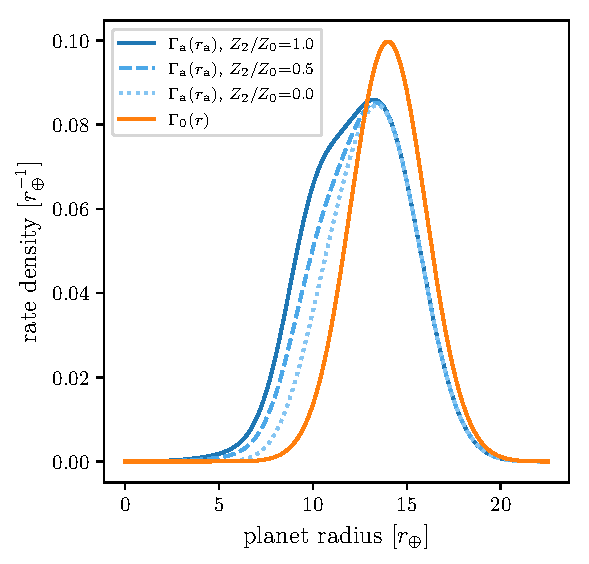
\includegraphics[width=.6\textwidth]{figures/int_rate_density_vs_radius_model_7_rpu_22.5_manyZs.pdf}
    \caption{
        Rate density for a population of planets with true radii $r$ drawn from
        $\mathcal{N}(14r_\oplus,2r_\oplus)$.
        This is similar to the hot Jupiter distribution presented 
        by~\citet{petigura_CKS_2017}.
    }
    \label{fig:gaussian_HJ}
\end{figure}


%%%%%%%%%%%%%%%%%%%%%%%%%%%%%%%%%%%%%%%%%%%%%%%%%%%%%%%%%%%%%%%%%%%%%%%%%%%%%%%
%%%%%%%%%%%%%%%%%%%%%%%%%%%%%%%%%%%%%%%%%%%%%%%%%%%%%%%%%%%%%%%%%%%%%%%%%%%%%%%
%\section{Discussion}
\label{sec:discussion}

\paragraph{Does a detected planet orbit the primary or secondary?}
Ciardi et al. (2015) studied the effects of stellar multiplicity on the 
planet radii derived from transit surveys.
They modeled the problem for {\it Kepler}\ objects of interest by matching a 
population of binary and tertiary companions to KOI stars, 
under the assumption that the KIC-listed stars were the primaries.
They then computed planet radius correction factors assuming that {\it 
Kepler}-detected planets orbited the primary or companion stars
with equal probability (their Sec. 5).
Under these assumptions, they found that any given planet's radius is on 
average underestimated by a multiplicative factor of 1.5.

Our models show that assuming a detected planet has equal probability of 
orbiting the primary or secondary leads to an overstatement of
binarity's population-level effects.
A planet orbiting the secondary does lead to extreme corrections, but these 
cases are rare outliers, because the searchable volume for secondaries is so 
much smaller than that for primaries.
Phrased in terms of the completeness, in our Model \#3 only $\sim 6\%$ of 
selected secondaries are searchable, compared to $\sim 60\%$ of selected 
primaries.
This means that when high-resolution imaging discovers a binary companion in 
system that hosts a detected transiting planet, the planet is much
more likely to orbit the primary.
This statement is independent of the fact that planets are often confirmed to 
orbit the primary by inferring the stellar density from the transit duration.


\paragraph{On the utility for future occurrence rate measurements}
Though they will be difficult to distinguish from false positives, {\it TESS}\ 
is expected to discover over $10^4$ giant planets (Sullivan et al. 2015).
One possible use of this overwhelmingly large sample will to measure an
occurrence rate of short-period giant planets.
Our work indicates that if this measurement is to be more precise than $\sim 
30\%$, binarity cannot be neglected.


\paragraph{What about {\it Kepler}?}
Barclay \& Collaborator (in preparation) have performed the exercise 
of taking stars selected by the {\it Kepler}\ team, pairing them with a 
population of secondaries, injecting a realistic distribution of planet radii, 
and then comparing the inferred occurrence rates with the true ones.
In their model, they find that binarity leads to an inferred rate of 
Earth-sized planets $\approx 10\%$ less than the true rate.
In our Model \#3, if all $\Lambda_i$'s are equal (a plausible assumption in 
the lack of evidence to the contrary), the underestimate is by 16\%.


\section{Discussion}
\label{sec:discussion}


\paragraph{How has binarity been considered in occurrence rate measurements?}
This study has shown that under a reasonable set of simplifying assumptions, 
ignoring binarity introduces systematic errors to star and planet counts in 
transit surveys, which then bias derived occurrence rates.
Thus far, real-world occurrence rate calculations\footnote{
    A list of occurrence rate papers is maintained at 
    \url{https://exoplanetarchive.ipac.caltech.edu/docs/occurrence_rate_papers.html}
} using transit survey data have mostly ignored stellar 
multiplicity~\citep[\textit{e.g.},][]{howard_planet_2012,fressin_false_2013,foreman-mackey_exoplanet_2014,dressing_occurrence_2015,burke_terrestrial_2015}.
For {\it Kepler} occurrence rates specifically, 
it seems that no one has yet carefully assessed binarity's importance, or lack 
thereof.
While we do not resolve the problem, we do suggest the approximate scale of 
the possible errors in a survey-independent manner.

Of course, on a system-by-system level stellar multiplicity affects the 
interpretation of planet candidates. High resolution imaging 
campaigns have measured the multiplicities of almost all {\it Kepler}\ Objects 
of Interest 
\citep{howell_speckle_2011,adams_adaptive_2012,adams_adaptive_2013,horch_observations_2012,
    horch_most_2014,lillo-box_multiplicity_2012,lillo-box_high-resolution_2014,dressing_adaptive_2014,
    law_robotic_2014,cartier_revision_2015,everett_high-resolution_2015,gilliland_hubble_2015,
    wang_influence_2015,wang_influence_2015-1,baranec_robo-ao_2016,ziegler_robo-ao_2017}.
The results of these programs have been collected 
by~\citet{furlan_kepler_2017}, and they represent an important advance in 
understanding the KOI 
sample's multiplicity statistics.
In particular, they can be immediately applied to rectify binarity's effects 
on the mass-radius diagram~\citep{furlan_densities_2017}.

This high resolution imaging campaign is also beginning to connect with
occurrence rate calculations.
The most recent rate studies have used~\citet{furlan_kepler_2017}'s 
catalog to test the effects of removing KOI hosts with known companions, which 
helps reduce contamination in the ``numerator'' of 
the occurrence rate (\citealt{fulton_california-_2017}; 
\citealt{petigura_CKS_2017}).
However, without an understanding of the multiplicity statistics of the 
non-KOI stars, the true number of searchable stars, and thus the true 
occurrence rates, will remain biased.

\paragraph{Practical effects: smooth detection efficiencies; finite SNR floors}
To interpret whether the results of this study are of any help for removing 
binarity's effects from the {\it Kepler}\ planet sample, a few practical 
concerns become pressing.

First, our calculations have ignored the fact that any given transit survey's 
finite SNR floor might censor the apparent rate density.
If the surveyed stars all have the same size, this is equivalent to 
saying that there might be a cutoff in apparent planet radii, below which no 
planets are detected.
The effects on our main results (e.g., 
Figs.~\ref{fig:occ_rate_model_3_log},~\ref{fig:frac_model_3}, 
and~\ref{fig:gaussian_HJ}) would be that the apparent rate density 
below the cutoff in apparent radius would simply drop to zero.

A second assumption we used is that the detection efficiency is a 
step function in SNR.
The detection efficiencies of real transit survey pipelines are smooth 
functions in SNR; see for example the injection \& recovery simulations 
performed by~\citet{christiansen_measuring_2016} on {\it Kepler}\ data, 
and the resulting smooth functional form adopted 
by~\citet{fulton_california-_2017}.
If we were to take a smooth detection probability in SNR, we would need to 
include a detection efficiency term in 
Eq.~\ref{eq:defn_apparent_rate_density} to inversely weight for planets 
with low probabilities of being detected.

The simplest way to avoid the conceptual complications of accounting for 
finite detection efficiency is to raise the SNR floor, to {\it e.g.,} 
${\rm SNR} \approx 12$ for {\it Kepler} 
(\citealt{fulton_california-_2017}, Fig.~5).
To a good approximation, this allows one to use the boolean distinctions 
``searchable'' and ``not searchable'' for signals of an observed depth (at 
fixed orbital period).
This also makes the survey strictly SNR-limited, rather than ``fuzzily 
SNR-limited''.
Since this threshold is set in an arbitrary manner anyway\footnote{For 
example, {\it Kepler}'s threshold of ${\rm SNR}=7.1$ was set for there to be 
no more than one statistical false alarm across the full {\it Kepler} 
campaign~\citep{jenkins_tests_2002}. Equally valid would have been to insist 
on no more than $10^{-3}$ false alarms per survey, raising the detection floor.
}, this simplification would put occurrence rate studies on 
clearer conceptual 
ground, and facilitate the process of converting the observed distributions
of apparent radii into true radius distributions.

\begin{comment}
If one insists on using a smooth detection efficiency, then life probably 
becomes more complicated.
It might then be necessary to model the detection pipeline's efficiency while 
somehow marginalizing over binarity.
Since the relative number of detections (at fixed $\delta_{\rm obs}$) coming 
from singles, primaries, and secondaries changes as a function of the 
intrinsic distribution of planet parameters (Fig.~\ref{fig:frac_model_3}), 
some complicated deconvolution might be required.
\end{comment}


\paragraph{The rate of Earth analogs}
Per {\it Kepler}'s primary science objective, the rate of Earth-like planets 
orbiting Sun-like stars has been independently measured by 
\citet{youdin_exoplanet_2011,petigura_prevalence_2013,dong_fast_2013,
    foreman-mackey_exoplanet_2014}, and \citet{burke_terrestrial_2015}.
These efforts have found that the one-year terrestrial planet occurrence rate 
varies between $\approx 0.03$ and $\approx 1$ per Sun-like star, depending on 
assumptions that are made when retrieving the rate 
(\citealt{burke_terrestrial_2015}'s Fig.~17).
In the power law model of Sec.~\ref{sec:model_3}, we noted that the inferred 
rate can be up to 50\% higher than the true rate around single stars.
Though this bias seems large, it is currently small compared to the other 
systematic factors that dominate the dispersion in $\eta_\oplus$ 
measurements.
If a future analyses determine absolute values of $\eta_\oplus$ to 
better than a factor of two, binarity might merit closer attention.

One relevant caveat to our assessment of binarity's importance for 
$\eta_\oplus$ measurements is that none of our models 
included the rate density's period-dependence. However, close binaries usually
provoke dynamical instabilities, leading to fewer long-period planets per 
star~\citep[\textit{e.g.},][]{holman_long-term_1999,wang_influence_2014,
    kraus_impact_2016}.
This effect might further affect transit survey measurements of $\eta_\oplus$
beyond our rough estimate.


\paragraph{The hot Jupiter rate discrepancy}
There is at least one context in which ignoring binarity has been suggested as 
a possible source of discrepant occurrence rate measurements.
Hot Jupiter occurrence rates measured by transit surveys ($\approx 0.5\%$) are 
marginally lower than those found by radial velocity surveys ($\approx 1\%$; 
see Table~\ref{tab:hj_rates}).
Though the discrepancy has weak statistical significance ($<3\sigma$),
one reason to expect a difference is that the corresponding stellar 
populations have distinct metallicities.
As argued by \citet{gould_frequency_2006}, the RV sample is biased towards 
metal-rich stars, which have been measured by RV surveys to preferentially 
host more giant 
planets~\citep{santos_spectroscopic_2004,fischer_planet-metallicity_2005}.
Investigating the discrepancy from the metallicty 
angle,~\citet{guo_metallicity_2017} measured the
{\it Kepler} field's mean metallicity to be $[{\rm M/H}]_{\rm Kepler}= 
-0.045\pm0.009$, which is lower than the California Planet Search's mean of 
$[{\rm M/H}]_{\rm CPS}= -0.005\pm0.006$.
The former value agrees with that measured by \citet{dong_metallicities_2014}.
Refitting for the metallicity exponent in $\Lambda_{\rm HJ} \propto 10^{\beta 
[{\rm M/H}] }$, \citeauthor{guo_metallicity_2017}\! found $\beta = 2.1\pm 
0.7$, and noted that this would imply that the metallicity difference could 
account for a $\approx 20\%$ relative difference in the measured rates between 
the CKS and {\it Kepler}\ samples~--~not a factor of two\footnote{
\citet{petigura_CKS_2017} recently found $\beta = 3.4^{0.9}_{-0.8}$.
This gives an $\approx 25\%$ relative difference, indicating metallicity could 
account for about half of the ``hot Jupiter rate discrepancy''.
}.
\citeauthor{guo_metallicity_2017}\! concluded that ``other factors, such as 
binary contamination and imperfect stellar properties'' must also be at play.

Aside from surveying stars of varying metallicities, radial velocity and 
transit surveys differ in how they treat binarity.
Radial velocity surveys typically reject both visual and spectroscopic binaries
\citep[\textit{e.g.},][]{wright_frequency_2012}.
Transit surveys typically observe binaries, but the question of whether they 
were searchable to begin with is left for later interpretation.
In spectroscopic follow-up of candidate transiting planets, the prevalence of 
astrophysical false-positives may also lead to a bias against confirmation of 
transiting planets in binary systems.

Ignoring these complications, in this work we showed that
binarity biases transit survey occurrence rates through its effects on 
star counts and the apparent radii of detected planets.
Our results from Sec.~\ref{sec:model_3} indicate that binarity 
could lead to underestimated HJ rates relative to singles by a multiplicative 
factor of at most $\approx 1.13$ (assuming a power-law radius distribution, 
and that no secondaries host HJs).
We later pointed out in Sec.~\ref{sec:further_models} that assuming a 
power-law radius distribution is probably wrong if one wishes to study the HJ 
rate discrepancy. If we instead assumed a 
Gaussian radius distribution~\citep[following][]{petigura_CKS_2017}, apparent 
HJ rates are actually {\it greater} 
than the true rate around singles.
\begin{comment}
If we believe the assumed power-law radius distribution, we can ask whether 
this ``correction factor'' might help resolve the discrepancy.
Explicitly, we ask: what is the probability of \citet{wright_frequency_2012}'s 
result, given a rate drawn from the stated bounds of~\citet{petigura_CKS_2017}?
In other words, we first take the true HJ rate per thousand stars as 
$\Lambda_{\rm HJ} = 5.7 \pm 1.3$, with Gaussian uncertainties. 
We then draw from a Poisson distribution and compute the probability of 
detecting at least 10 hot Jupiters in a sample of 836 stars.
Without accounting for binarity or metallicity, only 4\% of RV surveys would 
detect at least 10 hot Jupiters.
If we multiply $\Lambda_{\rm HJ}$ by $1.2$ to account 
for~\citet{guo_metallicity_2017}'s measured metallicity difference between the 
{\it Kepler}\ field and the local solar neighborhood, 9\% of RV surveys would 
detect at least 10 hot Jupiters.
If we multiply once more by $1.13$ to account for binarity's supposed bias, we 
find that 14\% of RV surveys would detect at least 10 hot Jupiters, still 
suggesting a weak discrepancy.

This suggestion should be taken with caution, because it (likely incorrectly) 
assumes a power-law radius distribution.
\end{comment}
This means that assuming a Gaussian similar to that reported 
by~\citet{petigura_CKS_2017}, binarity is unlikely to resolve the HJ rate 
discrepancy.
Of course, such calculations can be at most suggestive~--~a true resolution 
of binarity's effects may require a detailed understanding of the 
{\it Kepler}\ field's multiplicity statistics, and the mission's completeness 
(both for candidate detection and follow-up).
For instance, if hot Jupiters are less likely to be confirmed in binary 
systems, this might bias the rates low.


\paragraph{Fraction of detected planets with binary companions vs. apparent 
radius}
A prediction of Fig.~\ref{fig:frac_model_3} is that the fraction of detected 
planets with binary companions increases by $\approx 6-12\%$ going from 
$2r_\oplus$ to $\approx 1.4r_\oplus$.
In \citet{ziegler_robo-ao_2017}'s recent summary of the Robo-AO KOI survey, 
they reported the fraction of planet-hosting stars with Robo-AO detected 
companion stars, binning by Earths ($r\a < 1.6r_\oplus$), Neptunes 
($1.6r_\oplus < r\a < 3.9 r_\oplus$), Saturns ($3.9r_\oplus < r\a < 9 
r_\oplus$), and Jupiters ($r\a > 9r_\oplus$).
The reported nearby star rates and their $1\sigma$ uncertainties are:
\begin{itemize}
    \item Earths: $16.3 \pm 1.0\%$, from 1480 systems.
    \item Neptunes: $13.0 \pm 0.8\%$, from 2058 systems.
    \item Saturns: $13.6 \pm 2.0\%$, from 338 systems.
    \item Jupiters: $19.0 \pm 2.8\%$, from 247 systems.
\end{itemize} 
where the uncertainties were calculated 
following~\citet{burgasser_binarity_2003}.
The absolute values of the rates are less than the $\sim 45\%$ typical for 
Sun-like stars at least in part because of Robo-AO's sensitivity 
(\citealt{ziegler_robo-ao_2017}'s Fig.~2;~\citealt{raghavan_survey_2010}).
Another reason for the lower measured companion rates could be that planetary 
systems are less likely to have 
binary companions (as~\citealt{kraus_impact_2016} argued for close binary 
companions).
The uptick in the companion rate for Jupiters is likely tied to a large 
astrophysical false positive rate~\citep{santerne_sophie_2012}.
Going from Neptunes to Earths, the data suggest a weak increase in the 
detected planet companion fraction, perhaps of a few percent.


\paragraph{Does a detected planet orbit the primary or secondary?}
\citet{ciardi_understanding_2015} studied the effects of stellar multiplicity 
on the planet radii derived from transit surveys.
They modeled the problem for {\it Kepler}\ objects of interest by matching a 
population of binary and tertiary companions to KOI stars, 
under the assumption that the KIC-listed stars were the primaries.
They then computed planet radius correction factors assuming that {\it 
    Kepler}-detected planets orbited the primary or companion stars
with equal probability (their Sec.~5).
Under these assumptions, they found that any given planet's radius is on 
average underestimated by a multiplicative factor of $\approx\! 1.5$.
\citet{ziegler_robo-ao_2017} recently reported a similar mean radius 
correction factor for the multiple systems observed by the Robo-AO KOI survey, 
using the same assumption that detected planets are as likely to orbit the 
primary and the secondary.

Assuming a broken power-law radius distribution, we showed in 
Fig.~\ref{fig:frac_model_3} that assuming a detected planet has equal 
probability of orbiting the primary or secondary probably is rarely correct.
A planet orbiting the secondary does lead to extreme corrections.
However, at $r\a \gtrsim 2r_\oplus$, these cases are rare outliers.
At $r_\oplus \lesssim r\a \lesssim 2r_\oplus$, for all of the trial values of 
$Z_2/Z_0$ assumed in Fig.~\ref{fig:frac_model_3}, a detected planet is always 
more likely to orbit the primary than the secondary.
Only at very small apparent radii, $r\a \approx 0.5r_\oplus$, and only if 
secondaries host as many planets as singles and primaries, does this norm 
break down.

Of course, our model's assumptions (see the list in Sec.~\ref{sec:conclusion}) 
might not apply to the {\it Kepler}\ dataset.
If they do, then for the $56\%$ of ``\texttt{CONFIRMED}'' 
KOIs\footnote{Exoplanet Archive; \cite{akeson_nasa_2013}; 
\url{exoplanetarchive.ipac.caltech.edu}} with 
apparent radii $>2r_\oplus$, 
whenever high-resolution imaging 
discovers a binary companion in 
a system that hosts a detected transiting planet, the planet is much
more likely to orbit the primary.
This statement is independent of the fact that planets are often confirmed to 
orbit the primary by inferring the stellar density from the transit duration.


\paragraph{Utility in future occurrence rate measurements}
{\it TESS}\ is expected to discover over $10^4$ giant 
planets~\citep{ricker_transiting_2014,sullivan_transiting_2015}.
Though they will be difficult to distinguish from false positives, one 
possible use of this large sample will to measure an occurrence rate of 
short-period giant planets with minimal error from counting statistics.
Our models suggest that binarity will only become an appreciable fraction of 
the error budget at the $\approx 10\%$ precision level.
This should be sufficient for a rate measurement precise enough to indicate a 
preference between $\approx 0.5\%$ and $\approx 1\%$ of Sun-like stars hosting 
hot Jupiters.

\begin{comment}
\paragraph{Independent approaches for estimating binarity's effects}
T. Barclay et al.\! (in preparation) have performed the exercise of taking 
stars selected by the {\it Kepler}\ team, pairing them with a population of 
secondaries, injecting a realistic distribution of planet radii, 
and then comparing the inferred occurrence rates with the true ones.
In their model, they find that binarity leads to an inferred rate of 
Earth-sized planets $\approx 10\%$ less than the true rate.
In our Model \#3, if all $Z_i$'s are equal (a plausible assumption in 
the lack of evidence to the contrary), the underestimate is by a comparable 
16\%.
\end{comment}

%%%%%%%%%%%%%%%%%%%%%%%%%%%%%%%%%%%%%%%%%%%%%%%%%%%%%%%%%%%%%%%%%%%%%%%%%%%%%%%
%%%%%%%%%%%%%%%%%%%%%%%%%%%%%%%%%%%%%%%%%%%%%%%%%%%%%%%%%%%%%%%%%%%%%%%%%%%%%%%
%\section{Conclusion}
\label{sec:conclusion}

This study presented three simple models for the effects of binarity on 
occurrence rates measured by transit surveys.
The most realistic of these models (Model \#3) suggests that binarity does 
lead to underestimates in transit survey occurrence rates, but with less than 
$30\%$ relative error.
The model further suggests that hot Jupiter rates measured by transit surveys 
are biased to infer $\approx 1.3\times$ fewer hot Jupiters per star than 
surveys that only measure occurrence rates about single stars ({\it 
i.e..,} radial velocity surveys).
It also indicates that binarity's effects on the measured 
occurrence rates of Earth-sized planets are far smaller than current 
systematic uncertainties.
Though our models are simplistic, their agreement with Barclay \& 
Collaborator's recent detailed simulations indicate that they may capture the 
essential ingredients.


\section{Conclusion}
\label{sec:conclusion}

This study presented simple models for how binarity affects occurrence 
rates measured by transit surveys.
The simplest of these models (Sec.~\ref{sec:simplest}) provided an 
order-of-magnitude estimate that showed we would need very high twin binary 
fractions for binarity to affect apparent occurrence rates by more than 
$\sim$factors of two.

We then gave a general formula for the apparent rate density inferred by an 
observer ignoring binarity (Eq.~\ref{eq:general_Gamma_a}).
As input, this equation requires a volume-limited mass ratio distribution 
$f(q)$, and also the true rate densities for planets around singles, 
primaries, and secondaries.
The assumptions that make the model tractable are:
\begin{enumerate}
    \item the transit survey is SNR-limited;
    \item the true properties of all the singles and primaries are known to 
    the observer;
    \item the observers assume that binaries have the same properties as the 
    primaries;
    \item there are functions $L(M)$ and $R(M)$ that specify a star's 
    luminosity and radius in terms of its mass.
\end{enumerate}
Allowing for these conditions, many results follow:
\begin{itemize}
%
\item Assuming a power-law planet radius distribution, and that the same 
number of planets orbit singles, primaries, and secondaries, binarity 
influences apparent planet occurrence rates around Sun-like stars at the 
$\sim$few percent level from radii $2r_\oplus \lesssim r\a \lesssim 
17r_\oplus$ (Sec.~\ref{sec:model_2}).
%
\item Assuming a broken-power law planet radius distribution, with 
\citet{howard_planet_2012}'s exponent at $r > 2r_\oplus$ and a constant 
occurrence at $r < 2r_\oplus$, there is a ``bump'' in the apparent rate 
density at $r\a < 2r_\oplus$, leading to a relative error $\delta \Gamma_0 = 
|\Gamma_0 - \Gamma\a|/\Gamma_0$ of at most $\approx 50\%$ 
(Fig.~\ref{fig:occ_rate_model_3_log}).
Although this is smaller than current systematic uncertainties on the 
occurrence rates of Earth-sized planets, this means that binarity could
eventually become an important component of the $\eta_\oplus$ error budget.
%
\item Binarity ``fills in'' gaps in the radius distribution 
(Fig.~\ref{fig:model_4}), by an amount that could affect precise measurements 
of the depth, width, and slope of \citet{fulton_california-_2017}'s radius 
gap, in the event that planets are not carefully vetted with high resolution 
imaging.
%
\item Binarity does not lead to smaller apparent HJ occurrence rates 
(Fig.~\ref{fig:gaussian_HJ}).
This assumes a Gaussian planet radius distribution, similar to that reported 
by~\citet{petigura_CKS_2017}.
\end{itemize}

All of these results should be understood as only being strictly applicable 
when the assumptions listed above are met.
Otherwise, while it is only suggestive, our approach still provides 
helpful hints at how stellar binarity influences transit survey occurrence 
rates.





\acknowledgements{
It was a pleasure sharing discussions about this study with F. Dai and T. 
Barclay.
This work made use of NASA's Astrophysics Data System Bibliographic Services.

\software{\texttt{numpy}~\citep{walt_numpy_2011}, 
\texttt{scipy}~\citep{jones_scipy_2001}, 
\texttt{matplotlib}~\citep{hunter_matplotlib_2007}, 
\texttt{pandas}~\citep{mckinney-proc-scipy-2010}
}
}

\newpage
\appendix
\section{Derivation of general formula for apparent occurrence rate}
\label{sec:appendix}
Recall our definition of apparent rate density 
(Eq.~\ref{eq:defn_apparent_rate_density}).
Let us explicitly write $\pp=r$ and $\ps=M$; $R$ and $L$ are uniquely 
determined from the assumed stellar mass--radius--luminosity relation. We 
neglect the dependence on planetary orbital period.
The planets with $(r\a, M\a)$ are associated with 
systems of many different planetary and stellar properties, so $n_{\rm 
det}(r\a, M\a)$ is given by the convolution of the true rate density, 
$\Gamma(r, M)$, and $\mathcal{N}(r\a, M\a; r, M)$, the number (per 
unit $(r\a, M\a)$) of searchable stars that give $(r\a, M\a)$  when 
the true system actually has $(r, M)$. Mathematically,
\begin{align}
n_{\rm det}(r_a, M_a) &=
\sum_i n_{\rm det}^i(r_a, M_a) \\
&=
\sum_i \int \mathrm{d}r \mathrm{d}M \,
\mathcal{N}_{\rm s}^i(r_a,M_a; r,M)
\cdot\Gamma_i(r,M) \cdot p_{\rm tra}(r,M),
\label{eq:n_det}
\end{align}
where $i$ specifies the type of true host stars (0: single, 1: primary, 2: 
secondary).
The problem reduces to the evaluation of
\begin{equation}
\mathcal{N}_{\rm s}^i(\pp\a,\ps\a; \pp, \ps)
\end{equation}
for planets around single stars, primaries in binaries, and secondaries in 
binaries. 

\paragraph{Single stars} For $i=0$, 
\begin{equation}
\mathcal{N}_{\rm s}^0(r\a,M\a; r,M)
=\delta(r\a-r)\delta(M\a-M) N\s^0(r,M),
\end{equation}
so
\begin{equation}
n_{\rm det}^0(r\a, M\a)=N\s^0(r\a,M\a)\cdot \Gamma_0(r\a, 
M\a) \cdot p_{\rm tra}(r\a, M\a).
\end{equation}

\paragraph{Primaries in binaries}
The number of primaries with apparent parameters $(r_a,M_a)$ given the 
true parameters $(r,M)$ is
\begin{equation}
\mathcal{N}_{\rm s}^1(r_a, M_a; r, M)
=\int \mathrm{d}q\,f(q)\mathcal{N}_{{\rm s}, q}^1(r_a, M_a, q; r, M),
\label{eq:fancyN_s_1}
\end{equation}
where $f(q)$ is the volume-limited binary mass ratio distribution.

Since we assume $\ps\a=\ps_1$,
\begin{equation}
\mathcal{N}_{{\rm s},q}^1(r_a, M_a, q; r, M) \propto \delta(M_a-M).
\end{equation}
In this case, $\mathcal{N}_{{\rm s},q}^1$ is non-zero only at 
$r_a=R_a\sqrt{\delta_{\rm obs}}$, 
and the observed depth is
\begin{equation}
\delta_{\rm obs}
= \left[{r\over R(M_a)}\right]^2\times {L(M_a) \over L_{\rm sys}(M_a, q)}
\equiv \left[{r\over R(M_a)}\right]^2\times \mathcal{A}(q,M\a)^2
\label{eq:delta_obs_primaries} 
\end{equation}
The normalization of $\mathcal{N}_{{\rm s},q}^1$ is given by the number of 
binaries that are searchable for a signal $\delta_{\rm obs}$ and that have the 
mass ratio $q$:
\begin{equation}
N_{\rm s}^0(\delta_{\rm obs}, 
L(M_a))\cdot
{n_b\over n_s}\left[L_{\rm sys}(M_a, q) \over L(M\a)\right]^{3/2}
=N_{\rm s}^0(\delta_{\rm obs}, L(M_a))
\cdot \frac{{\rm BF}}{1 - {\rm BF}} \cdot {1 \over \mathcal{A}(q,M\a)^3}.
\label{eq:primary_normalization}
\end{equation}

Thus,
\begin{align}
\notag
\mathcal{N}_{{\rm s}, q}^1(r_a, M_a, q; r, M)
&=N_{\rm s}^0(\delta_{\rm obs}, L(M_a))
\cdot \frac{{\rm BF}}{1 - {\rm BF}} \cdot {1 \over \mathcal{A}(q,M\a)^3}\\
&\times\delta \left[r_a-r\mathcal{A}(q,M\a)\right]\delta(M_a-M).
%&=N_{\rm s}^0(\delta_{\rm obs}, L(M_a))\cdot\mu(\mathrm{BF},M_a)\\
%&\times\delta \left(r_a-r\sqrt{{L(M_a) \over L_{\rm sys}(M_a, 
%q)}}\right)\delta(M_a-M).
\label{eq:N_s_1}
\end{align}


\paragraph{Secondaries in binaries}
In this case, $M=qM_1=qM_a$, so
\begin{equation}
\mathcal{N}_{{\rm s},q}^2(r_a, M_a, q; r, M)
\propto \delta\left(M_a-{M\over q}\right).
\label{eq:fancyN_s_2_prop}
\end{equation}
Again $\mathcal{N}_{\rm s}^2$ is non-zero only at $r_a=R_a\sqrt{\delta_{\rm 
        obs}}$, but this 
time
\begin{equation}
\delta_{\rm obs} = \left[{r\over R(qM_a)}\right]^2 \times {L(qM_a) 
    \over L_{\rm sys}(M_a, q)}.
\end{equation}
The normalization remains the same as the previous case (we are counting the 
searchable stars at a given observed depth $\delta_{\rm obs}$, total 
luminosity of the binary is the same).
Thus,
\begin{equation}
\mathcal{N}_{\rm s}^2(r_a, M_a; r, M)
=\int \mathrm{d}q\,f(q)\mathcal{N}_{{\rm s}, q}^2(r_a, M_a, q; r, M),
\end{equation}
where
\begin{align}
\notag
\mathcal{N}_{\rm s}^2(r_a, M_a; r, M; q)
&=N_{\rm s}^0(\delta_{\rm obs}, L(M_a)) \cdot \frac{{\rm BF}}{1 - {\rm BF}} 
\cdot {1 \over \mathcal{A}(q,M\a)^3}\\
&\times \delta \left(r_a-r\sqrt{ \left[{R(M_a)\over R(qM_a)}\right]^2 
    {L(qM_a) 
        \over L_{\rm sys}(M_a, q)} }\right)\delta\left(M_a-{M\over q}\right).
\label{eq:mathcal_N_s_2}
\end{align}

One might worry in Eq.~\ref{eq:mathcal_N_s_2} that we opt to write 
$\mathcal{N}\s^2 \propto \delta(M_a - M/q)$, rather than $\propto \delta(M_a q 
- M)$ or some other delta function with the same functional dependence, 
but a different normalization once integrated.
We do this because the delta function in Eq.~\ref{eq:mathcal_N_s_2} is 
defined with respect to the measure ${\rm d}M\a$, not ${\rm d}M$.
This is because $\mathcal{N}\s^2$ is defined as a number per $r\a$, per $M\a$.

\paragraph{Number of detected planets}
Marginalizing per Eq.~\ref{eq:n_det}, we find
\begin{align}
\notag
n_{\rm det}^0(r\a, M\a)
&=\int\mathrm{d}r\mathrm{d}M\,\mathcal{N}_{\rm s}^0(r\a, M\a; r, M)
\cdot\Gamma_0(r, M) \cdot p_{\rm tra}(M)\\
&=N\s^0(\delta_{\rm obs}, L(M\a))\cdot\Gamma_0(r\a, M\a) \cdot p_{\rm 
    tra}(M\a),
\label{eq:n_det_0}
\end{align}
and
\begin{align}
\notag
n_{\rm det}^1(r\a, M\a)
&=\int\mathrm{d}r\mathrm{d}M\,\mathcal{N}_{\rm s}^1(r\a, M\a; r, M)
\cdot\Gamma_1(r, M) \cdot p_{\rm tra}(M)\\
&=N\s^0(\delta_{\rm obs}, L(M\a))\cdot p_{\rm tra}(M\a) \cdot
{\mathrm{BF}\over{1-\mathrm{BF}}} \int {\mathrm{d}q \over 
    \mathcal{A}^4}\,f(q)\,\Gamma_1\left({r_a\over\mathcal{A}}, M\a\right),
\label{eq:n_det_1}
\end{align}
where
\begin{equation}
\mathcal{A}(q, M\a)=\sqrt{L(M\a) \over L_{\rm sys}(M\a, q)}.
\end{equation}
Finally,
\begin{align}
n_{\rm det}^2(r\a, M\a)
&=\int\mathrm{d}r\mathrm{d}M\,\mathcal{N}_{\rm s}^2(r\a, M\a; r, M)
\cdot\Gamma_2(r, M) \cdot p_{\rm tra}(M)\\
&=
N\s^0(\delta_{\rm obs}, L(M\a))\cdot \frac{{\rm BF}}{1 - {\rm BF}}
\int {q \mathrm{d}q \over 
{\mathcal{A}^3\mathcal{B}}}\,f(q)\,\Gamma_2(r_a/\mathcal{B}, 
qM\a)\,p_{\rm 
    tra}(qM\a),
\label{eq:n_det_2}
\end{align}
where
\begin{equation}
\mathcal{B}(q, M\a)={R(M\a)\over R(qM\a)}\sqrt{{L(qM\a) \over L_{\rm 
            sys}(M\a, q)} }.
\end{equation}


\paragraph{General formula for apparent occurrence rate}
Using the results above, the apparent rate density,
\begin{align}
\Gamma\a(r\a,M\a) &= 
\frac{1}{N_{\rm s,a}(r\a,M\a) p_{\rm tra}(r\a,M\a)} \times
\sum_i n_{\rm det}^i (r\a,M\a),
\end{align}
evaluates to

\begin{align}
\notag
\Gamma\a(r\a,M\a) &= {1\over 1+\mu(\mathrm{BF}, M\a)}\times
\left\{ \Gamma_0(r\a, M\a)+ 
\frac{{\rm BF}}{1 - {\rm BF}}
\left[ \int {\mathrm{d}q \over \mathcal{A}^4}\,f(q)\,\Gamma_1\left({r\a\over 
    \mathcal{A}}, 
M\a\right)\,
\right.   
\right. \\
& \quad\quad\quad\quad\quad \left.\left.
+\int {q \mathrm{d}q \over 
    {\mathcal{A}^3\mathcal{B}}}\,f(q)\,\Gamma_2\left({r\a\over 
    \mathcal{B}}, 
qM\a\right)\,
{R(qM\a) \over R(M\a)}
q^{-1/3} \right]	\right\}.
\end{align}
This equation is used to derive Eqs.~\ref{eq:model5_apparent_rate_density} 
and~\ref{eq:powerlaw_vary_binary}, and is numerically integrated to create 
Figs.~\ref{fig:occ_rate_model_3_log},~\ref{fig:model_4}, 
and~\ref{fig:gaussian_HJ}.
It is validated in limits in which it is possible to write down the answer 
(e.g., Eq.~\ref{eq:model_1_apparent_rate_density}), and also against a Monte 
Carlo realization of the twin binary models (Secs.~\ref{sec:model_1} 
and~\ref{sec:model_2}).


\newpage
%% \begin{deluxetable}{} command tell LaTeX how many columns
%% there are and how to align them.
\begin{deluxetable}{cccc}
    
%% Keep a portrait orientation

%% Over-ride the default font size
%% Use Default (12pt)

%% Use \tablewidth{?pt} to over-ride the default table width.
%% If you are unhappy with the default look at the end of the
%% *.log file to see what the default was set at before adjusting
%% this value.

%% This is the title of the table.
\caption{Occurrence rates of hot Jupiters (HJs) about FGK dwarfs, as measured 
by radial velocity and transit surveys.}
\label{tab:hj_rates}

%% This command over-rides LaTeX's natural table count
%% and replaces it with this number.  LaTeX will increment 
%% all other tables after this table based on this number
\tablenum{1}

%% The \tablehead gives provides the column headers.  It
%% is currently set up so that the column labels are on the
%% top line and the units surrounded by ()s are in the 
%% bottom line.  You may add more header information by writing
%% another line between these lines. For each column that requries
%% extra information be sure to include a \colhead{text} command
%% and remember to end any extra lines with \\ and include the 
%% correct number of &s.
\tablehead{\colhead{Reference} & \colhead{HJs per thousand stars} & 
\colhead{HJ Definition} 
%& 
%\colhead{} \\ 
%    \colhead{} & \colhead{(planets per thousand stars)} & \colhead{} & 
%    \colhead{}
} 

%% All data must appear between the \startdata and \enddata commands
\startdata
Marcy+ 2005 & 12$\pm$1 & $a<0.1\,{\rm AU}; P\lesssim10\,{\rm day}$ \\
Cumming+ 2008 & 15$\pm$6 & -- \\
Mayor+ 2011 & 8.9$\pm$3.6 & -- \\
Wright+ 2012 & 12.0$\pm$3.8 & -- \\
Gould+ 2006 & $3.1^{+4.3}_{-1.8}$ & $P<5\,{\rm day}$ \\
Bayliss+ 2011 & $10^{+27}_{-8}$ & $P<10\,{\rm day}$ \\
Howard+ 2012 & 4$\pm$1 & $P<10\,{\rm day}; r_p=8-32r_\oplus$; solar 
subset\tablenotemark{a} \\
-- & 5$\pm$1 & solar subset extended to $Kp<16$ \\
-- & 7.6$\pm$1.3 & solar subset extended to $r_p>5.6r_\oplus$. \\
Moutou+ 2013 & 10$\pm$3 & {\it CoRoT} average; $P\lesssim 10\,{\rm day}$, 
$r_p>4r_\oplus$  \\
Petigura+ (in prep) & 5.7$\pm$1.3 &
    $r_p=8-24r_\oplus$; $1<P/{\rm day}<10$; CKS stars\tablenotemark{b} \\
Santerne+ (in prep) & 9.5$\pm$2.6 & {\it CoRoT} galactic center \\
-- & 11.2$\pm$3.1 & {\it CoRoT} anti-center \\
\enddata

%% Include any \tablenotetext{key}{text}, \tablerefs{ref list},
%% or \tablecomments{text} between the \enddata and 
%% \end{deluxetable} commands

%% General table comment marker
\tablecomments{
    The upper four results are from radial velocity surveys; the rest
    are from transit surveys. Many of these surveys selected different 
    stellar samples. ``--'' denotes ``same as above''.
}
\tablenotetext{a}{
    Howard+ 2012's ``solar subset'' was defined as {\it Kepler}-observed stars 
    with $4100\,{\rm K}<T_{\rm eff}<6100\,{\rm K}$, $Kp <15$, $4.0 < \log g < 
    4.9$. Their rate selected planets with measured signal to noise $>10$.
    }
\tablenotetext{b}{
    Petigura+ (in prep)'s CKS subset included $\ldots$
}   
\end{deluxetable}



\newpage
\bibliographystyle{yahapj}                            
\bibliography{bibliography} 

\end{document}
